\pdfoutput=1
\documentclass[11pt,a4paper]{article}
\usepackage{abhijit-research}
\renewcommand{\PaperCode}{P01}
\renewcommand{\PaperKind}{RESEARCH PAPER}
\renewcommand{\PaperVersion}{VERSION 1.1}
\renewcommand{\PaperDate}{AUGUST 2026}
\renewcommand{\PaperTitle}{Future-Complete Quotients}
\renewcommand{\PaperSubtitle}{Recursive Distinction}
\renewcommand{\PaperFullTitle}{Future-Complete Quotients and Recursive Distinction}
\renewcommand{\PaperShortTitle}{Future-Complete Quotients}
\renewcommand{\PaperKeywords}{recursive distinction; predictive quotient; behavioural closure; finite reconstruction; reporter refinement}
\renewcommand{\PaperClassification}{The reconstruction, closure, refinement, finite quotient, and common-source results are theorem-level statements in the declared finite constructor. Interpretations beyond that constructor are stated separately.}
\renewcommand{\PaperCitation}{Singh, Abhijit. 2026. \textit{Future-Complete Quotients and Recursive Distinction}. Research manuscript, version 1.0.}
\begin{document}
\MakeResearchTitle
\MakeResearchContents
\MakeResearchAbstract{%
A finite source calculus is developed from one formal primitive: a distinction has a complete family of resultants, and every resultant may distinguish again. Finite unlabelled non-plane hierarchies retain containment, multiplicity, and complete resultant families. Complete recursive views and complete one-occurrence continuation decks reconstruct every finite source hierarchy. The central closure theorem characterizes exactly when a quotient reporter supports an autonomous continuation law: the complete reported response must be constant on every reporter fibre. Failure induces a least response-forced refinement; success implies stable blindness to every distinction erased by the quotient. The calculus further constructs least closed combinations of reporters, finite predictive quotients, target-free expansion systems, and common-source relations between incomparable perspectives. An occurrence-sensitive prime triad and its nine-state, thirty-six-relation realization are added as a concrete quotient-closure test.
}
\section{Introduction}

Any formal account of distinction begins after at least one distinction
has already been made. Terms such as \emph{state}, \emph{event},
\emph{set}, and \emph{operation} belong on the reportable side of that
boundary. The first task is therefore to mark where formal description
begins without representing the absence of description as one more
object.

We use \(P_{0}/R\) for that boundary. It denotes no reportable
distinction and is assigned no carrier, point, value, state, law,
temporal order, modality, or truth value. This is a constraint on the
theory's language rather than a claim about a hidden substrate. Every
symbol in the paper is already a distinction, so every proof and
computation belongs to \(P_{1}\), the first reportable perspective,
whose primitive separation is binary.

The sole source rule is

\[\mathsf{D}:\quad\quad\text{a distinction has resultants, and every resultant may distinguish.}\]

Completeness and recursion specify how the primitive is reported.
Completeness forbids the omission of a resultant; recursion permits the
same rule to act at any resultant. Neither introduces a clock,
probability, coordinate system, objective, or update schedule. A
complete \(q\)-resultant family written in \(P_{1}\) is consequently an
encoding of \(q\) retained occurrences. When \(q > 2\), indexing that
record by a hypothetical \(P_{q - 1}\) does not grant access to a native
nonbinary logic.

The least finite transcription that keeps containment, multiplicity, and
complete resultant families visible is an unlabelled, non-plane rooted
hierarchy. A record is either an unresolved terminal \(\bullet\), or a
containing occurrence with an unordered multiset of at least two child
records. Equal child descriptions may repeat: descriptive equality does
not cancel occurrence. The hierarchy is a declared representation within
\(P_{1}\), not an ontological identification of \(R\) with a tree.

Given a source hierarchy and a reporter \(Q\) that identifies some
source states, when does an operation on the source induce a law on the
reported states? The closure criterion answers this directly: two states
with the same report must have the same complete reported response.
Otherwise the reporter has merged states with incompatible futures.
Retaining the incompatibility, rather than choosing or averaging an
outcome, determines the least refinement needed to make the report
lawful.

Closure also fixes a limit. Once a law descends to a quotient, all of
its iterates remain functions of that quotient. The law cannot
reconstruct a distinction that its own state space consistently erased.
Thus autonomy and blindness are not separate phenomena in this calculus;
both are consequences of the same fibre condition.

The development proceeds from the finite hierarchy and its
reconstructive views to complete output decks, quotient closure, forced
refinement, and closed reporter combination. Later sections introduce
finite interaction systems, a target-free expansion process, and
common-source comparisons. These latter constructions carry additional
hypotheses and are kept separate from the primitive core.

\section{Principal results and
scope}

The central theorem may be stated without interpretive terminology:

\begin{quote}
\textbf{Complete-behaviour closure.} Let \(Q\) report the declared
finite hierarchies, whose complete occurrence decks are finite. A
single-valued continuation law descends to the \(Q\)-states if and only
if complete reported response is constant on every fibre of \(Q\). If
constancy fails, equality through all finite response depths defines the
least finer reporter on which every reported arity closes.
\end{quote}

The paper establishes five groups of results.

\begin{enumerate}
\def\labelenumi{\arabic{enumi}.}
\item
  \textbf{Source structure and reconstruction.} The declared hierarchy
  grammar transcribes complete recursive distinction. Within it, the
  containing occurrence is the unique unselected site at which one
  retained role persists through a distinction without deletion,
  duplication, or child selection. Complete recursive views reconstruct
  a hierarchy at finite depth, as does the deck formed by replacing
  every terminal occurrence once. Counts and flattened arity profiles
  are strictly coarser because they lose shared containment.
\item
  \textbf{Law, refinement, and stable loss.} The closure criterion is
  necessary and sufficient. Its failure determines a least
  response-forced refinement; its satisfaction proves stable blindness,
  since response iteration preserves the reporter's fibres.
  Grouping-depth reporters form a closed hierarchy, and the least closed
  combination of two reporters is obtained by closing their direct pair.
  This combination is associative and commutative up to fibres, with
  \(X \vee_{c}X \simeq {Cl}_{\infty}(X)\).
\item
  \textbf{Finite effect and interaction quotients.} On a declared finite
  carrier, an effect family induces the least same-referent quotient
  sufficient for those effects. For codomains with at least two values,
  properly finer reports admit strictly more compatible candidate laws.
  For \(|X| = q \geq 2\) and a pointed operation of arity \(m \geq 1\),
  finite interaction contexts generate the coarsest focus-preserving
  predictive quotient and stabilise after at most \(q - 2\) strict
  refinements.
\item
  \textbf{Test systems.} A target-free binary expansion process yields
  local replacement, name invariance, commutation at separate current
  occurrences, ancestry-restricted histories, exact continuation
  factorisation, and nontermination. A second construction separates
  histories, ordered forms, order-free forms, and availability, making
  the permanence of closed information loss explicit.
\item
  \textbf{Relations among perspectives.} For two quotients of a common
  source, direct translation exists exactly along refinement.
  Incomparable quotients are related through the source-induced
  relation; their joint quotient is the least report retaining both
  distinction families and may be strictly finer than either marginal.
\end{enumerate}

\section{Complete distinction and behavioural
closure}

\subsection{Formal boundary and
provenance}

The calculus begins with a restriction: its first inscription must not
be mistaken for a description of what precedes inscription. We therefore
separate the formal boundary from every object constructed beyond it.

\subsubsection{\texorpdfstring{3.1.1 The \(P_{0}/R\)
boundary}{3.1.1 The P\_\{0\}/R boundary}}

\textbf{Boundary statement.} \(P_{0}/R\) denotes no reportable
distinction. It is assigned no carrier or internal relation and is not
identified with a familiar mathematical object. Any such identification
would already distinguish that representation from alternatives, and so
would belong on the reportable side of the boundary.

The notation is eliminative, not descriptive: it marks the limit of
positive formal attribution. Even the sentence ``there is no reportable
distinction'' is written from a reportable perspective. It fixes the
provenance of the calculus rather than supplying a positive theory of
\(R\).

\subsubsection{The first reportable
perspective}

\textbf{Perspective convention.} \(P_{1}\) is the first reportable
perspective: one distinction with two resultants. Every word, equation,
diagram, proof, and program in this paper is consequently a \(P_{1}\)
inscription. The calculus cannot step outside that representational
condition to certify the native experience or mathematics of another
perspective.

A binary medium may nevertheless encode a finite family with \(q > 2\)
distinguishable occurrences. Accordingly, ``a \(q\)-resultant
distinction'' means precisely:

\begin{quote}
\(P_{1}\) records, without deleting an occurrence, a complete family of
\(q\) distinguishable resultants.
\end{quote}

This is an external \(P_{1}\) presentation, not a claim of access to a
native nonbinary perspective.

Figure 1 records this asymmetry: the boundary is not a source node,
while binary and higher-arity records are constructions on its
reportable side.

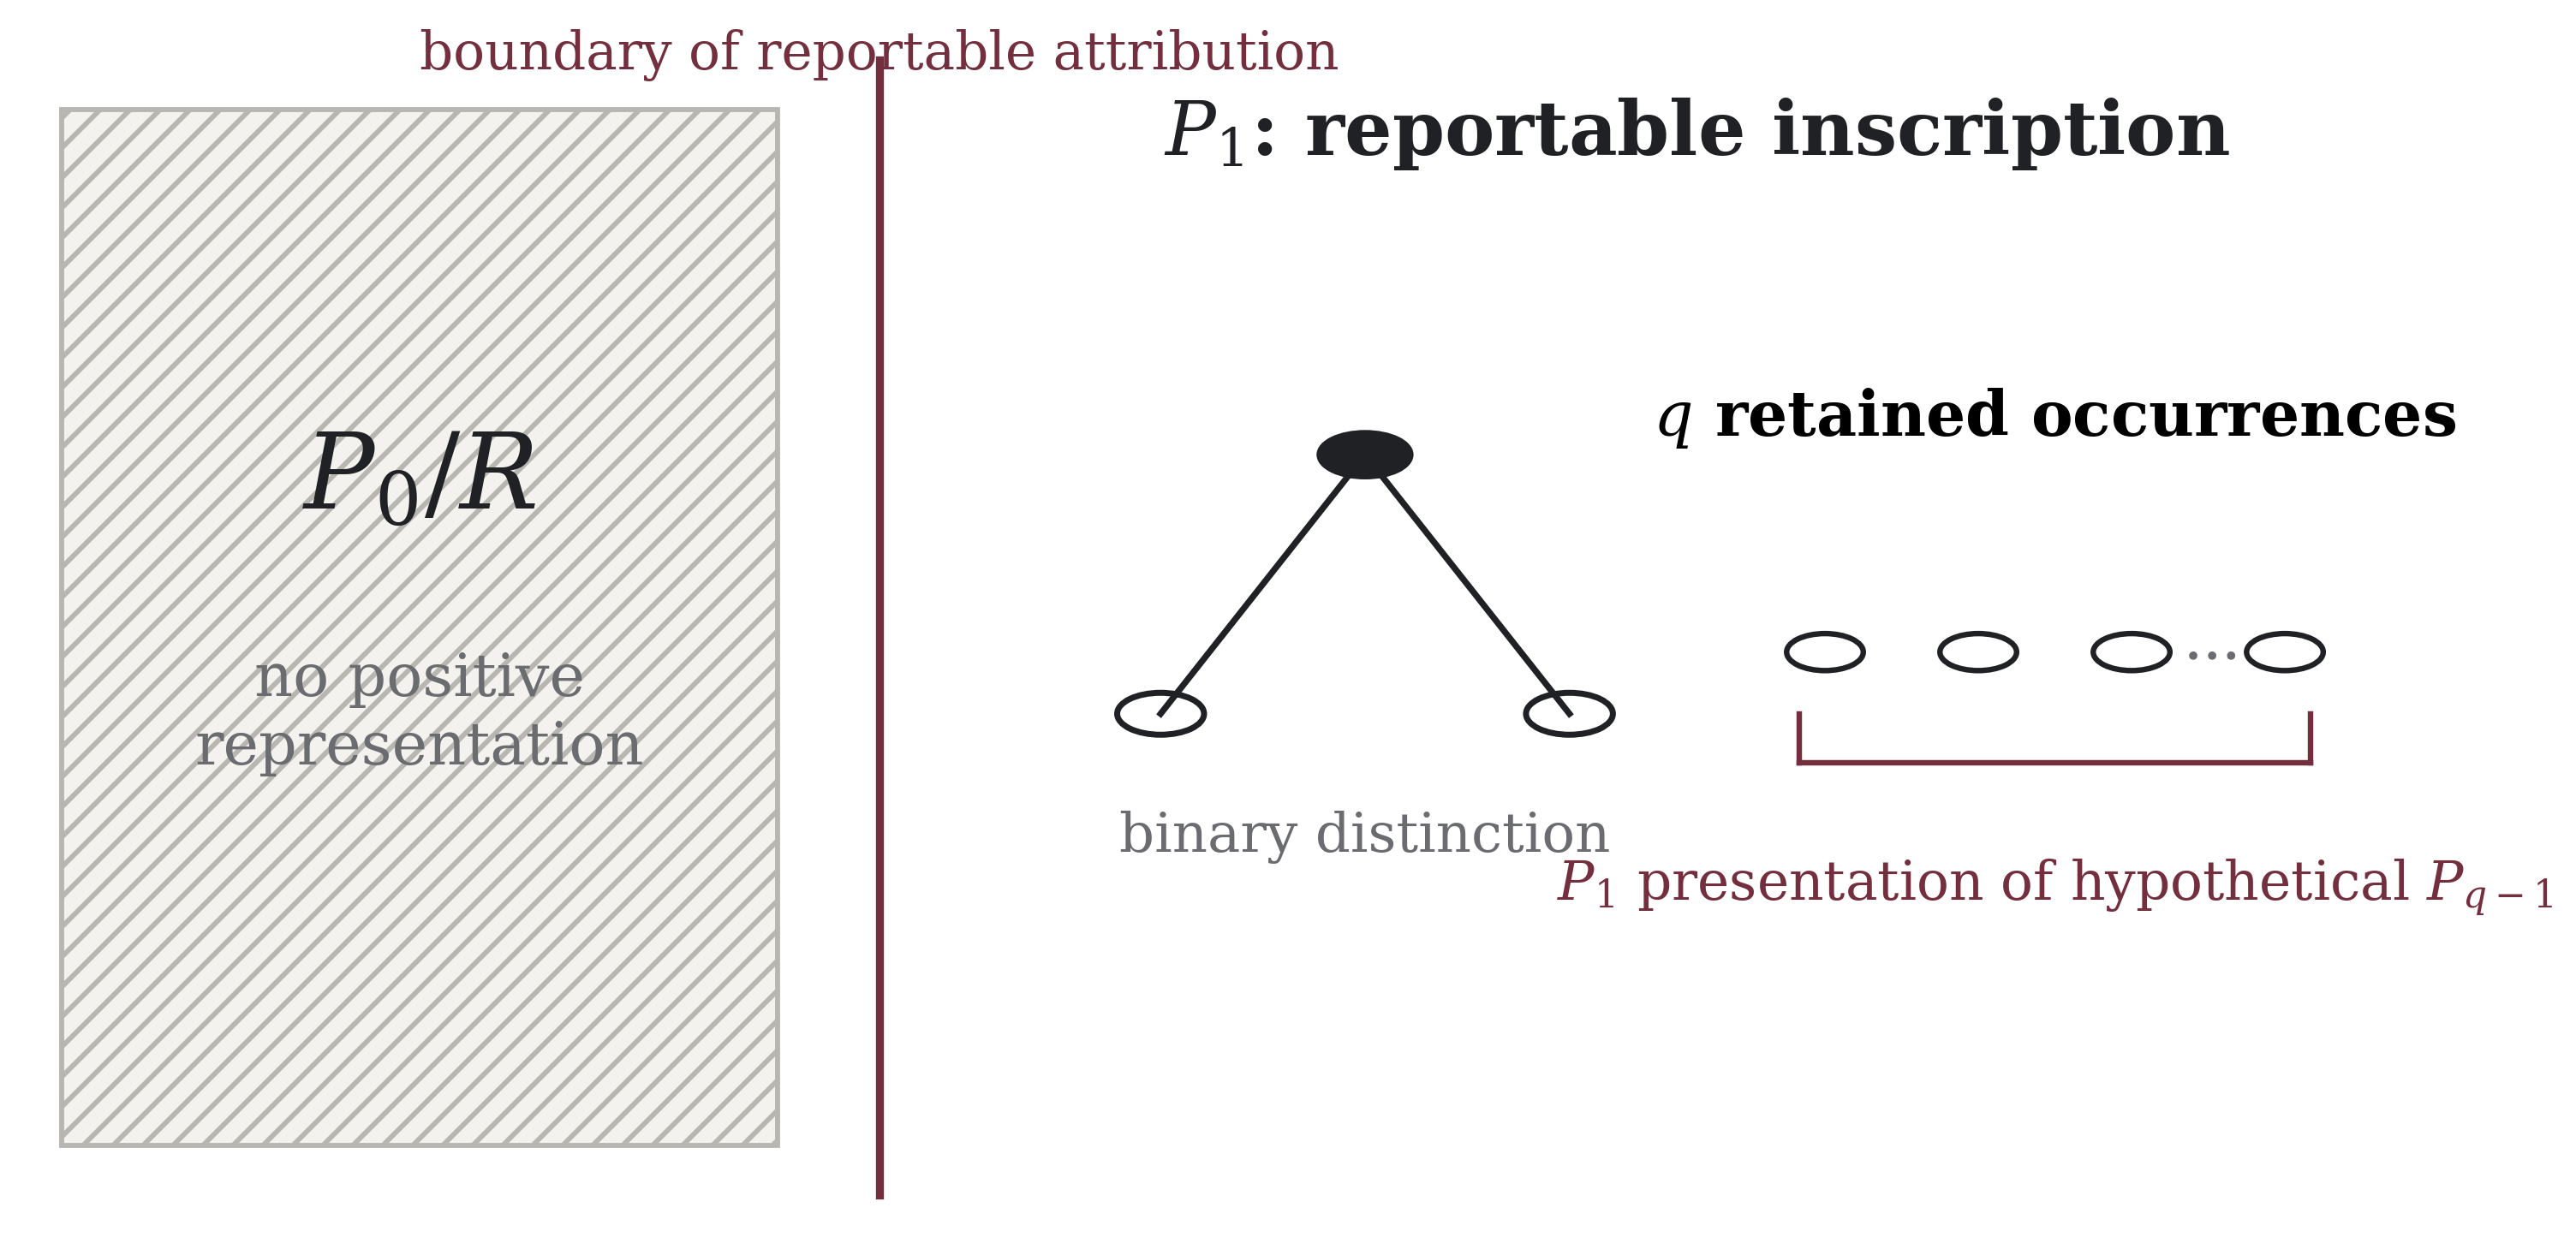
\includegraphics[width=6.12in,height=2.98268in]{figures/rId25.png}

Figure 1. Representation boundary and perspective indexing. The vertical
rule marks the limit of positive attribution; no transition is drawn
across it.

\subsubsection{The sole source rule}

The construction retains one source rule:

\[\boxed{\mathsf{D}:\quad\text{a distinction has resultants, and every resultant may distinguish.}}\]

Completeness means that no resultant is discarded from the report;
recursion means that the same rule is applied again to a resultant.
Neither adds a second source rule. In particular, \(\mathsf{D}\)
contains no scheduler, coordinates, probability law, metric,
conservation equation, logical valuation, or target phenomenon.

Definitions below specify the mathematical constructor; numbered
propositions, theorems, and corollaries state consequences of their
displayed hypotheses. Appendix A records their provenance.

\subsection{The minimal complete
hierarchy}

\subsubsection{Grammar and equality}

\begin{quote}
\textbf{Definition 3.2.1 (finite complete hierarchy).} Let
\(\mathcal{H}\) be generated by
\end{quote}

\[T:: = \bullet \quad\text{or}\quad\langle T_{1},\ldots,T_{q}\rangle,\quad\quad q \geq 2.\]

The symbol \(\bullet\) records a resultant with no further reported
distinction. The term \(\langle T_{1},\ldots,T_{q}\rangle\) records a
containing occurrence and all of its \(q\) present resultants. Children
are unordered, since \(\mathsf{D}\) supplies no order; equal
descriptions retain their occurrence multiplicity rather than being
identified.

Equality in \(\mathcal{H}\) is therefore isomorphism of finite
unlabelled, non-plane, rooted hierarchies with multiplicity. A node of
the underlying rooted hierarchy is called an \emph{occurrence}. An
occurrence is \emph{terminal} when it is represented by \(\bullet\), and
\emph{internal} when it carries a nonempty child family.

This grammar is minimal relative to four declared reporting obligations:

\begin{enumerate}
\def\labelenumi{\arabic{enumi}.}
\tightlist
\item
  a distinction leaves one containing occurrence at which it occurred;
\item
  every present resultant is retained;
\item
  every resultant may recursively carry the same form of record;
\item
  no child order or label is inserted without another supplied
  distinction.
\end{enumerate}

``Minimal'' is relative to these four obligations. The claim is not that
\(R\) is a hierarchy, but that \(\mathcal{H}\) is the least explicit
\(P_{1}\) transcription used here that records recursive containment and
the complete resultant family without introducing labels or order.

For \(T \in \mathcal{H}\), let \(L(T)\) be its number of terminal
occurrences and \(h(T)\) the maximum number of containment edges from
the root to a terminal. For an internal occurrence \(v\), let
\(q(v) \geq 2\) denote its arity. These are measurements of a completed
record, not source primitives.

We use finite multisets throughout. The notation
\(\{\{ a_{1},\ldots,a_{m}\}\}\) retains the number of occurrences of
each value; multiset equality includes multiplicity. If
\(f:A \rightarrow B\) and \(M\) is a finite multiset on \(A\), then
\(f_{*}M\) denotes its multiplicity-preserving pushforward.

\subsubsection{The information order on
reporters}

\begin{quote}
\textbf{Definition 3.2.2 (reporter and refinement).} A reporter on
\(\mathcal{H}\) is any function \(Q:\mathcal{H} \rightarrow X\). For
reporters \(X\) and \(Y\), write
\end{quote}

\[X \preccurlyeq Y\]

when equality of \(Y\)-reports implies equality of \(X\)-reports.
Equivalently, \(X\) factors through \(Y\). Thus \(Y\) retains every
distinction retained by \(X\), and perhaps more. Reporters are
identified \emph{up to fibres}: \(X \simeq Y\) means \(X(T) = X(U)\) if
and only if \(Y(T) = Y(U)\) for all \(T,U \in \mathcal{H}\).

The order compares retained distinctions only; it carries no independent
ranking by truth, observer quality, physical resolution, or temporal
progress.

\subsubsection{Why the containing occurrence
persists}

Suppose an occurrence carries one focal role \(x\). After it
distinguishes into a complete unlabelled family, the old role could
apparently be erased, assigned to one child, copied to every child, or
retained at the containing occurrence. The first choice violates
retention; the second introduces an unsupplied child selection; the
third turns one role into \(q\). Only the fourth preserves exactly one
focal role.

\begin{quote}
\textbf{Proposition 3.2.3 (unselected persistence).} Inside the declared
hierarchy transcription, the containing occurrence is the unique
placement that retains one old focal role through its distinction
without deleting, selecting, or duplicating that role.
\end{quote}

This is an identity principle of the transcription. It assigns no
objecthood or persistence to \(R\): the children form the complete new
resultant family, with no default heir to the old role.

\subsubsection{First invariants and the cost of
flattening}

The completed record supports exact accounting identities that are
absent from the source rule.

\begin{quote}
\textbf{Proposition 3.2.4 (balance).} Every \(T \in \mathcal{H}\)
satisfies
\end{quote}

\[\boxed{L(T) = 1 + \sum_{v\text{ internal}}^{}\left( q(v) - 1 \right).}\]

\emph{Proof.} The unresolved record \(\bullet\) has one terminal and no
internal contribution. Replacing one terminal by a family of \(q\)
resultants increases the terminal total by \(q - 1\) and adds one
internal occurrence contributing exactly \(q - 1\) to the displayed sum.
Every finite hierarchy is obtained by finitely many such replacements,
so induction on the number of internal occurrences proves the identity.
\(\ensuremath{\square}\)

For a homogeneous \(q\)-resultant hierarchy with \(I\) internal
occurrences, the balance reduces to

\[L = 1 + (q - 1)I.\]

For homogeneous binary hierarchies this becomes \(L = I + 1\). Both
identities belong to the finite \(P_{1}\) transcription.

Now put \(e_{v} = q(v) - 1\). Then

\[L(T) - 1 = \sum_{v}^{}e_{v}.\]

This scalar factors through two distinct losses:

\[\mathcal{H} \rightarrow \{\{ e_{v}\}\} \rightarrow \sum_{v}^{}e_{v} = L - 1.\]

The first arrow erases which internal occurrences contain which others.
The second erases even the multiset decomposition of the total excess.
To see the first loss directly, let \(T_{a,b}\) have \(a\) children at
the root and \(b\) children below each root child. Reversing the two
layers yields \(T_{b,a}\). For \(a \neq b\) their containment histories
differ, but both have \(ab\) terminals. The equality \(ab = ba\) is
therefore visible at the scalar shadow while the two complete
hierarchies remain distinct.

Flattening can lose information even when terminal total, root arity,
and the total number of grandchildren are all retained. Consider

\[A = \langle \bullet ,\langle \bullet , \bullet \rangle,\langle \bullet , \bullet , \bullet , \bullet \rangle\rangle\]

and

\[B = \langle \bullet ,\langle \bullet , \bullet , \bullet \rangle,\langle \bullet , \bullet , \bullet \rangle\rangle.\]

Both have seven terminals, three root children, and six grandchildren,
but their complete nested child-family reports are respectively

\[\{\{\varnothing,2\lbrack*\rbrack,4\lbrack*\rbrack\}\}\quad\text{and}\quad\{\{\varnothing,3\lbrack*\rbrack,3\lbrack*\rbrack\}\}.\]

Hence a flattened occurrence union does not determine recursive nesting.
An associativity law on a flat algebra may be perfectly sound, but the
quotient has changed the object under study: scalar and flat reporters
are proper shadows of the hierarchy.

\subsection{Complete present-resultant
views}

Two complete families will be used: the children present at an
occurrence, and the possible one-occurrence continuations of a terminal.
They are different constructions.

\subsubsection{Present-family
readout}

\begin{quote}
\textbf{Definition 3.3.1 (present-resultant operator).} For any
expression \(e\) evaluable on hierarchies, define
\end{quote}

\[\ensuremath{\llbracket}\Delta e\ensuremath{\rrbracket}( \bullet ) = \varnothing,\]

and

\[\ensuremath{\llbracket}\Delta e\ensuremath{\rrbracket}\left( \langle T_{1},\ldots,T_{q}\rangle \right) = \{\{ \ensuremath{\llbracket}e\ensuremath{\rrbracket}\left( T_{1} \right),\ldots,\ensuremath{\llbracket}e\ensuremath{\rrbracket}\left( T_{q} \right)\}\}.\]

Thus \(\Delta\) returns the entire present child multiset. It neither
selects nor labels a child, and it performs no ordering, averaging, or
scalarization.

\subsubsection{Recursive self-view}

Begin with one undifferentiated focal report

\[V_{0}(T) = *.\]

Apply the same report recursively to every present resultant:

\[V_{r + 1}( \bullet ) = (*,\varnothing),\]

\[V_{r + 1}\left( \langle T_{1},\ldots,T_{q}\rangle \right) = \left( *,\{\{ V_{r}\left( T_{1} \right),\ldots,V_{r}\left( T_{q} \right)\}\} \right).\]

Write

\[V_{\omega}(T): = \left( V_{r}(T) \right)_{r \geq 0},\]

so equality of \(V_{\omega}\)-reports means equality at every finite
view depth.

The first coordinate retains the focal role at its containing
occurrence. The second records the absence or presence of a child family
and, when present, applies the same reading to every child occurrence.

\begin{quote}
\textbf{Theorem 3.3.2 (finite reconstruction).} If \(T \in \mathcal{H}\)
has height \(h\), then \(V_{h + 1}(T)\) determines \(T\). Consequently,
equality through every finite view depth has exactly the equality fibres
of \(\mathcal{H}\):
\end{quote}

\[\boxed{V_{h(T) + 1}(T)\text{ reconstructs }T,\quad\quad V_{\omega} \simeq \mathcal{H}.}\]

\emph{Proof.} We induct on the height. If \(T = \bullet\), then
\(V_{1}(T) = (*,\varnothing)\), which identifies the terminal record.
Let \(T = \langle T_{1},\ldots,T_{q}\rangle\) have height \(h > 0\). Its
\(V_{h + 1}\)-report contains, with multiplicity, the family
\(\{\{ V_{h}\left( T_{1} \right),\ldots,V_{h}\left( T_{q} \right)\}\}\).
Every child has height at most \(h - 1\); by the induction hypothesis,
its \(V_{h}\)-report reconstructs it. Reconstruct every member of the
complete child multiset and place that multiset under the single
containing occurrence. This recovers \(T\). Because every finite \(T\)
has finite height, equality at all finite view depths implies equality
in \(\mathcal{H}\), while equality in \(\mathcal{H}\) plainly implies
equality of every view. \(\ensuremath{\square}\)

\begin{quote}
\textbf{Theorem 3.3.3 (strict view hierarchy).} Erasing the deepest
retained family from a \(V_{r + 1}\)-report yields its \(V_{r}\)-report,
so
\end{quote}

\[V_{0} \preccurlyeq V_{1} \preccurlyeq V_{2} \preccurlyeq \cdots.\]

Each refinement is strict on the unbounded family of finite hierarchies.

\emph{Proof.} The forgetful map is immediate from the recursive
definition. A terminal and an internal occurrence agree under \(V_{0}\)
and differ under \(V_{1}\). More generally, if \(T\) and \(U\) first
differ at view depth \(r + 1\), embed each beneath the same newly
supplied containing context; their first difference is shifted to depth
\(r + 2\). Hence examples witnessing strictness exist at every finite
level. \(\ensuremath{\square}\)

Here \(r\) counts nested applications of the \(P_{1}\) readout. It has
no assigned interpretation as time, distance, physical scale, knowledge,
computational complexity, or perspective index.

Reconstruction requires neither names nor child order. Complete
multiplicity and recursive containment suffice. Present-resultant access
is therefore faithful on finite hierarchies, whereas scalar count
identifies many nonisomorphic records.

\subsection{Complete one-occurrence future
decks}

\subsubsection{Definition and elementary
invariants}

Fix an externally reported arity \(q \geq 2\).

\begin{quote}
\textbf{Definition 3.4.1 (complete occurrence deck).} For
\(T \in \mathcal{H}\), let \(E_{q}(T)\) be the finite multiset obtained
by replacing each terminal occurrence of \(T\), one occurrence at a
time, by a \(q\)-resultant occurrence
\(\langle \bullet ,\ldots, \bullet \rangle\). If symmetric terminal
occurrences yield isomorphic outputs, the output hierarchy appears with
the corresponding multiplicity.
\end{quote}

The deck is an exhaustive family of one-occurrence continuations, not a
probability distribution. Each output \(U \in E_{q}(T)\) satisfies

\[L(U) = L(T) + q - 1,\]

and the total occurrence multiplicity of the deck is

\[\left| E_{q}(T) \right|_{occ} = L(T).\]

Where \(\Delta\) reads the current children of one focal occurrence,
\(E_{q}\) enumerates every terminal occurrence at which another
distinction can be recorded.

\subsubsection{Source reconstruction from one complete
deck}

\begin{quote}
\textbf{Theorem 3.4.2 (deck reconstruction).} For every fixed integer
\(q \geq 2\) and all finite \(T,U \in \mathcal{H}\),
\end{quote}

\[\boxed{E_{q}(T) = E_{q}(U) \Rightarrow T = U.}\]

\emph{Proof.} Let \(h = h(T)\). Expanding a terminal at depth \(h\)
creates an output of height \(h + 1\), while expanding any shallower
terminal creates an output of height at most \(h\). Hence the maximum
height among members of \(E_{q}(T)\) is \(h + 1\), and every
maximum-height member results from expansion at a maximum-depth
terminal.

Choose a maximum-height output \(W\). In the source \(T\), no internal
occurrence can lie at depth \(h\), since it would have a terminal
descendant below depth \(h\), contradicting maximality of \(h\).
Therefore \(W\) has exactly one internal occurrence at depth \(h\): the
newly inserted \(q\)-resultant occurrence. Contract that occurrence to a
terminal. The contraction uniquely recovers \(T\). Thus a complete deck
determines its source. Equal decks have a common maximum-height member
and reconstruct the same source, proving \(T = U\). \(\ensuremath{\square}\)

Thus the unquotiented one-step continuation family is faithful to the
full finite hierarchy, not merely to terminal count. Before passing to
quotients, the following subsection records the exact locality available
when two replacements occur on opposite sides of a retained cut. Section
3.5 then asks which parts of this continuation structure survive a
quotient report.

\subsubsection{Persistent cuts and restricted two-step
interaction}

Occurrence provenance permits an exact cut without choosing a child or
flattening either side. For a finite hierarchy \(T\), let \(\Lambda(T)\)
be its set of terminal occurrences. For a marked occurrence \(v\), write
\(D = T|_{v}\) for the subhierarchy rooted at \(v\) and
\(T = C\lbrack D\rbrack\) for the associated one-hole context. The
terminals below \(v\) form \(\Lambda_{v}(T) \subseteq \Lambda(T)\),
canonically identified with \(\Lambda(D)\). Write

\[\Lambda_{v}^{out}(T) = \{ u \in \Lambda(T):u \notin \Lambda_{v}(T)\}\]

for the terminal occurrences outside the marked subhierarchy. Let

\[B_{q} = \langle \bullet ,\ldots, \bullet \rangle,\quad\quad q \geq 2,\]

where the bracket contains exactly \(q\) terminal entries, and write
\(T\left\lbrack u \leftarrow B_{q} \right\rbrack\) for replacement of
the terminal occurrence \(u\) by \(B_{q}\). Define the
occurrence-indexed multisets

\[E_{q}^{in}(T;v) = \{\{ T\left\lbrack u \leftarrow B_{q} \right\rbrack:u \in \Lambda_{v}(T)\}\},\]

\[E_{q}^{out}(T;v) = \{\{ T\left\lbrack u \leftarrow B_{q} \right\rbrack:u \in \Lambda_{v}^{out}(T)\}\}.\]

Outputs that become isomorphic are aggregated only after their
originating terminal occurrences have been counted.

\begin{quote}
\textbf{Theorem 3.4.3 (persistent cut and exact reunion).} For every
finite \(T \in \mathcal{H}\), every marked occurrence \(v\), and every
integer \(q \geq 2\),
\end{quote}

\[\boxed{E_{q}(T) = E_{q}^{in}(T;v) \uplus E_{q}^{out}(T;v).}\]

Moreover,

\[E_{q}^{in}(T;v) = \{\{ C\lbrack W\rbrack:W \in E_{q}(D)\}\},\]

with multiplicity preserved. Every member of the inside deck retains the
outer context \(C\lbrack - \rbrack\), and every member of the outside
deck retains the marked subhierarchy \(D\) unchanged.

\emph{Proof.} Every terminal occurrence of \(T\) lies in exactly one of
the disjoint sets \(\Lambda_{v}(T)\) and \(\Lambda_{v}^{out}(T)\). The
definition of \(E_{q}(T)\) indexes one replacement by each terminal
occurrence, so this set partition induces the displayed multiset
disjoint union, including all multiplicities. Under the canonical
identification \(\Lambda_{v}(T) \cong \Lambda(D)\), replacing \(u\)
below \(v\) changes only \(D\) and yields
\(C\left\lbrack D\left\lbrack u \leftarrow B_{q} \right\rbrack \right\rbrack\);
this proves the inside-deck formula. A replacement outside
\(\Lambda_{v}(T)\) is disjoint from the marked occurrence and therefore
leaves \(D\) unchanged. \(\ensuremath{\square}\)

The cut also isolates an exact, deliberately local order-independence
result.

\begin{quote}
\textbf{Theorem 3.4.4 (opposite-side commutation).} Let
\(T = C\lbrack D\rbrack\) and \(v\) be as above. Fix integers
\(q,r \geq 2\). For every \(u \in \Lambda_{v}(T)\) and
\(w \in \Lambda_{v}^{out}(T)\), both terminal occurrences survive when
the other is replaced, and
\end{quote}

\[\boxed{T\left\lbrack u \leftarrow B_{q} \right\rbrack\left\lbrack w \leftarrow B_{r} \right\rbrack = T\left\lbrack w \leftarrow B_{r} \right\rbrack\left\lbrack u \leftarrow B_{q} \right\rbrack.}\]

Consequently, the complete occurrence-indexed two-step multiset obtained
by a \(q\)-replacement inside the cut followed by an \(r\)-replacement
outside is equal to the multiset obtained in the opposite order.

\emph{Proof.} The terminal occurrences \(u\) and \(w\) are distinct and
lie in disjoint occurrence regions. Replacing \(u\) changes only the
subhierarchy at \(u\), so \(w\) remains a terminal occurrence with the
same provenance; symmetrically, replacing \(w\) leaves \(u\) available.
Both composites are therefore the simultaneous hierarchy obtained from
\(T\) by inserting \(B_{q}\) at \(u\) and \(B_{r}\) at \(w\). Pairing
the two orderings by the same occurrence pair \((u,w)\) is a bijection
of their finite indexing sets and preserves the resulting hierarchy.
Aggregating isomorphic outputs thus preserves equal multiplicities.
\(\ensuremath{\square}\)

The restriction to opposite sides of a retained cut is essential.
Identical or nested occurrences require a separate interaction analysis.
This result supplies a concrete two-step law at source level; the
quotient criterion below decides whether any reporter retains enough
information for that law, or any complete continuation law, to descend.

\subsection{Autonomous quotient
laws}

A reporter may retain less than the full hierarchy. The pertinent
question is whether its reported state determines its complete reported
behaviour.

Let \(Q:\mathcal{H} \rightarrow X\) be any declared reporter. For a deck
\(E_{q}(T)\), define its pushed report

\[Q_{*}E_{q}(T) = \{\{ Q(W):W \in E_{q}(T)\}\},\]

with occurrence multiplicity retained.

\begin{quote}
\textbf{Definition 3.5.1 (autonomous} \(q\)\textbf{-law).} An autonomous
continuation law for \(Q\) at arity \(q\) is a function
\end{quote}

\[F_{Q,q}:Q\left( \mathcal{H} \right) \rightarrow MFin\left( Q\left( \mathcal{H} \right) \right)\]

such that

\[F_{Q,q}\left( Q(T) \right) = Q_{*}E_{q}(T)\]

for every \(T \in \mathcal{H}\). Here \(MFin(X)\) denotes finite
multisets on \(X\).

Thus an autonomous law is internal to the reporter: the present
\(Q\)-state determines the complete multiset of next \(Q\)-states
without reference to a hidden representative in \(\mathcal{H}\).

\begin{quote}
\textbf{Theorem 3.5.2 (autonomy/closure criterion).} An autonomous
\(q\)-law exists if and only if the complete pushed deck is constant on
every \(Q\)-fibre:
\end{quote}

\[\boxed{Q(T) = Q(U) \Rightarrow Q_{*}E_{q}(T) = Q_{*}E_{q}(U)\quad\text{for all }T,U \in \mathcal{H}.}\]

\emph{Proof.} If \(F_{Q,q}\) exists and \(Q(T) = Q(U) = x\), then

\[Q_{*}E_{q}(T) = F_{Q,q}(x) = Q_{*}E_{q}(U),\]

so the condition is necessary. Conversely, suppose the condition holds.
For \(x \in Q\left( \mathcal{H} \right)\), choose any \(T\) with
\(Q(T) = x\) and define \(F_{Q,q}(x) = Q_{*}E_{q}(T)\). Fibre constancy
makes this definition independent of the representative, so it is a
function satisfying the required equation. \(\ensuremath{\square}\)

Figure 2 separates the two cases of Theorem 3.5.2: descent when complete
decks agree on every fibre, and refinement when they do not.

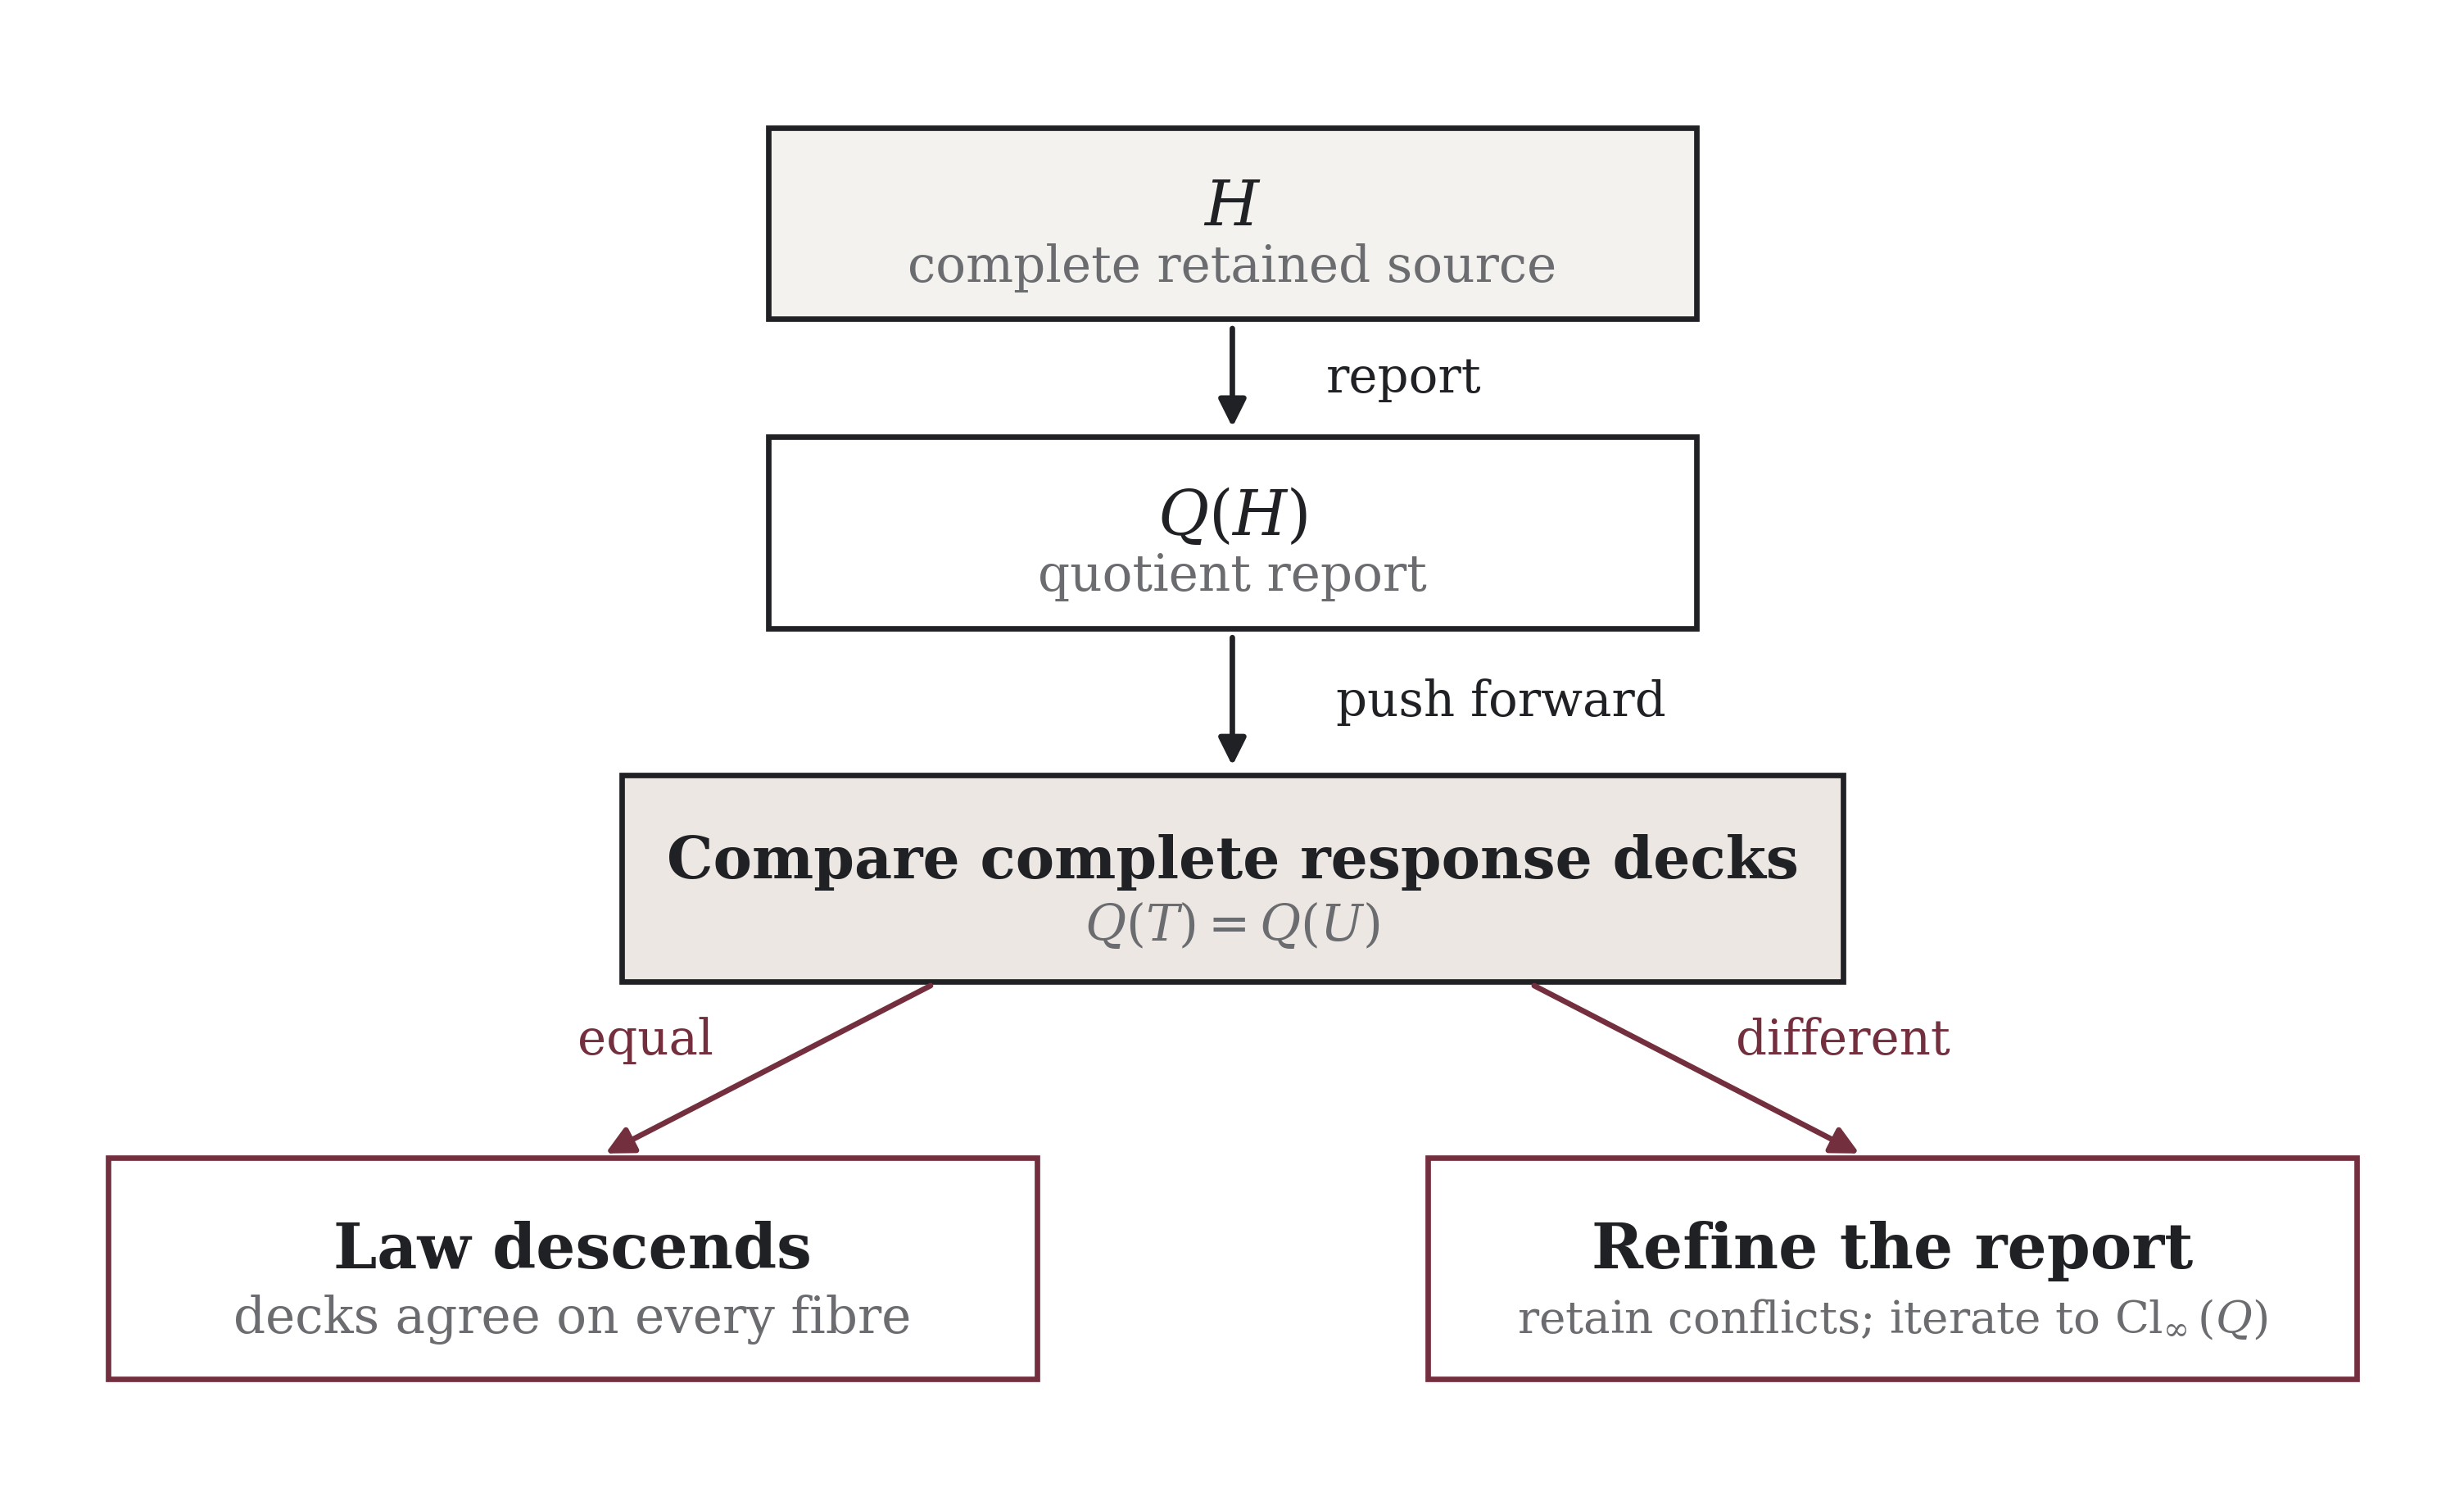
\includegraphics[width=6.12in,height=3.70496in]{figures/rId43.png}

Figure 2. Complete-behaviour closure. Fibre constancy yields an
autonomous quotient law; conflicting decks force the least refinement
that retains every behaviourally relevant distinction.

We call \(Q\) \(q\)\emph{-closed} when it satisfies the criterion, and
\emph{all-arity closed} when it is \(q\)-closed for every integer
\(q \geq 2\).

If closure fails, the complete response at a fibre is the set of all
decks it supports:

\[{\widehat{F}}_{Q,q}(x) = \{ Q_{*}E_{q}(T):Q(T) = x\}.\]

This set-valued family is not an autonomous single-valued law. Its
plurality records one precise fact: \(Q\) has erased a distinction on
which its complete response depends. No probabilistic or stochastic
interpretation follows without additional structure.

\begin{quote}
\textbf{Corollary 3.5.3 (count forced by complete multiplicity).} Every
\(q\)-closed reporter \(Q\) refines terminal count \(L\).
\end{quote}

\emph{Proof.} If \(Q(T) = Q(U)\), closure gives equal pushed decks.
Equal finite multisets have equal total multiplicity. These
multiplicities are respectively \(L(T)\) and \(L(U)\), hence
\(L(T) = L(U)\). \(\ensuremath{\square}\)

Terminal count is itself all-arity closed, because its complete law is

\[L \mapsto L\text{ occurrences of }L + q - 1.\]

Therefore \(L\) is the coarsest reporter closed under complete terminal
replacement with occurrence multiplicity. The result is
operation-relative: count is not sufficient for \(\Delta\), whose
recursive views reconstruct the full hierarchy.

The identity reporter is closed. So is the multiset of arity excesses
\(\{\{ q(v) - 1\}\}\): a \(q\)-replacement appends \(q - 1\), while the
current excess sum fixes deck multiplicity by Proposition 3.2.4.
Internal-node count \(I\), by contrast, is not closed when multiplicity
is retained. A binary star and a ternary star both have \(I = 1\), but
their decks contain two and three occurrences, respectively. Its first
response refinement is exactly \((I,L)\), which is closed: every
replacement sends \((I,L)\) to \((I + 1,L + q - 1)\) with multiplicity
\(L\).

Accordingly, a reporter may already be autonomous, may acquire finitely
many missing coordinates, or may require an unbounded refinement tower.
The criterion decides which case occurs from the reported behaviour
itself.

\subsection{Response-forced
completion}

When closure fails, the conflicting responses identify which fibres must
split. Iterating this observation gives a canonical completion without
prescribing target classes.

\subsubsection{Iterated response
reporters}

Fix a reporter \(Q:\mathcal{H} \rightarrow X\). Define

\[R_{0}^{Q}(T) = Q(T).\]

Recursively, let \(R_{r + 1}^{Q}(T)\) retain \(R_{r}^{Q}(T)\) together
with, for every integer \(q \geq 2\), the complete multiplicity deck of
\(R_{r}^{Q}\)-reports of members of \(E_{q}(T)\):

\[R_{r + 1}^{Q}(T) = \left( R_{r}^{Q}(T),(R_{r*}^{Q}E_{q}(T))_{q \geq 2} \right).\]

Only equality fibres matter; no canonical code for the arity-indexed
tuple is needed. Let \(T \equiv_{r}^{Q}U\) mean
\(R_{r}^{Q}(T) = R_{r}^{Q}(U)\). Since \(R_{r + 1}^{Q}\) retains
\(R_{r}^{Q}\),

\[\equiv_{r + 1}^{Q}\  \subseteq \  \equiv_{r}^{Q}.\]

Define the limiting equivalence

\[T \equiv_{\infty}^{Q}U\quad \Leftrightarrow \quad T \equiv_{r}^{Q}U\text{ for every finite }r.\]

Write \({Cl}_{\infty}(Q)\) for the quotient reporter whose fibres are
the \(\equiv_{\infty}^{Q}\)-classes.

\subsubsection{Least-closure theorem}

\begin{quote}
\textbf{Theorem 3.6.1 (least all-response closed refinement).} On the
finite hierarchy family \(\mathcal{H}\), \({Cl}_{\infty}(Q)\) is
all-arity closed. Moreover, it is the least discriminating all-arity
closed reporter that refines \(Q\). Explicitly:
\end{quote}

\begin{enumerate}
\def\labelenumi{\arabic{enumi}.}
\tightlist
\item
  \(Q \preccurlyeq {Cl}_{\infty}(Q)\);
\item
  \({Cl}_{\infty}(Q)\) is \(q\)-closed for every \(q \geq 2\);
\item
  if \(S\) is all-arity closed and \(Q \preccurlyeq S\), then
  \({Cl}_{\infty}(Q) \preccurlyeq S\).
\end{enumerate}

\emph{Proof.} The first statement follows because \(R_{0}^{Q} = Q\) is
retained at every later depth.

For closure, suppose \(T \equiv_{\infty}^{Q}U\) and fix \(q \geq 2\).
The occurrence decks \(E_{q}(T)\) and \(E_{q}(U)\) are finite. For each
\(r \geq 0\), equality of \(R_{r + 1}^{Q}(T)\) and \(R_{r + 1}^{Q}(U)\)
implies equality of the complete \(R_{r}^{Q}\)-decks. Hence there exists
a multiplicity-preserving bijection between the occurrence-indexed
members of \(E_{q}(T)\) and \(E_{q}(U)\) that pairs outputs having equal
\(R_{r}^{Q}\)-reports.

Let \(\Pi_{r}\) be the finite set of all such bijections. Each
\(\Pi_{r}\) is nonempty. Since equality at depth \(r + 1\) implies
equality at depth \(r\), the sets descend:

\[\Pi_{0} \supseteq \Pi_{1} \supseteq \Pi_{2} \supseteq \cdots.\]

They are subsets of the one finite set of all bijections between the two
finite occurrence decks. A descending sequence of nonempty subsets of a
finite set has nonempty intersection. Choose
\(\pi \in \bigcap_{r}\Pi_{r}\). Every output is paired by \(\pi\) with
an output equal under every finite \(R_{r}^{Q}\), hence equal under
\(\equiv_{\infty}^{Q}\). The pushed \({Cl}_{\infty}(Q)\)-decks are
therefore equal. Since \(q\) was arbitrary, the limiting reporter is
all-arity closed.

For leastness, let \(S\) be any all-arity closed reporter refining
\(Q\), and suppose \(S(T) = S(U)\). We prove by induction on \(r\) that
\(R_{r}^{Q}(T) = R_{r}^{Q}(U)\). The base case follows from
\(Q \preccurlyeq S\). Assume the assertion holds at depth \(r\) for
every pair of equal \(S\)-reports. Because \(S\) is \(q\)-closed,
equality \(S(T) = S(U)\) gives, for every \(q \geq 2\), a
multiplicity-preserving pairing of \(E_{q}(T)\) and \(E_{q}(U)\) whose
paired outputs have equal \(S\)-reports. By the induction hypothesis
those paired outputs have equal \(R_{r}^{Q}\)-reports. Hence the
complete \(R_{r}^{Q}\)-decks agree for every \(q\), and
\(R_{r + 1}^{Q}(T) = R_{r + 1}^{Q}(U)\). Induction yields equality at
all finite response depths, so \(T \equiv_{\infty}^{Q}U\). Thus equality
under \(S\) implies equality under \({Cl}_{\infty}(Q)\), which is
exactly \({Cl}_{\infty}(Q) \preccurlyeq S\). \(\ensuremath{\square}\)

The universal property is relative to the stated carrier and operation:
finite hierarchies, complete one-terminal replacement at every reported
arity, and multiplicity-preserving decks.

Restricting the constructor to a fixed \(q \geq 2\) gives, by the same
proof, the least \(q\)-closed refinement \({Cl}_{q}(Q)\). A reporter can
be closed for one replacement arity and fail for another; the all-arity
completion is the common refinement obtained when every reported arity
is retained.

In the preceding closure proof, finiteness is used when the descending
family of compatible pairings is shown to have a common member. Although
\(\mathcal{H}\) is infinite, no uniform finite stabilisation depth is
asserted. Infinite occurrence decks would require an additional
compactness or choice principle.

Two states separate at the first response depth where their complete
behaviour differs, and later separations occur only when subsequent
responses reveal another conflict. State refinement and autonomous law
are therefore determined together.

\subsection{Stable blindness}

\subsubsection{The ceiling theorem}

Response completion repairs unstable loss. It cannot recover an erasure
already compatible with every supported response.

\begin{quote}
\textbf{Theorem 3.7.1 (stable blindness).} If \(Q\) is all-arity closed,
then for every finite \(r \geq 0\),
\end{quote}

\[\boxed{R_{r}^{Q}(T) = R_{r}^{Q}(U)\quad \Leftrightarrow \quad Q(T) = Q(U).}\]

Consequently, \({Cl}_{\infty}(Q) \simeq Q\).

\emph{Proof.} Because \(R_{r}^{Q}\) retains \(Q\), equality of
\(R_{r}^{Q}\)-reports implies equality of \(Q\)-reports. For the
converse, proceed by induction. It is immediate for \(r = 0\). Suppose
\(R_{r}^{Q}\) is a function of \(Q\). Since \(Q\) is closed,
\(Q(T) = Q(U)\) implies that for each \(q \geq 2\) the occurrence decks
\(E_{q}(T)\) and \(E_{q}(U)\) can be paired with equal \(Q\)-reports.
Applying the inductive functional dependence to paired outputs gives
equal \(R_{r}^{Q}\)-reports, so the complete \(R_{r}^{Q}\)-decks agree.
Together with equality of the retained first coordinate, this gives
\(R_{r + 1}^{Q}(T) = R_{r + 1}^{Q}(U)\). Thus every \(R_{r}^{Q}\) is
both a function of \(Q\) and a refinement retaining \(Q\), so their
fibres agree. \(\ensuremath{\square}\)

Erased distinctions may remain in \(\mathcal{H}\); the theorem says that
iteration of the autonomous \(Q\)-law supplies no behavioural witness
for them. Unequal responses expose unstable erasure, while closure makes
the erasure stable under the observed operation.

This yields a sharp ceiling. The views \(V_{r}\) reconstruct because
\(\Delta\) retains recursive child grouping. A closed scalar or flat
reporter may erase that relation while retaining a perfectly autonomous
replacement law; further iteration then cannot restore it.

Stable blindness is thus an invariant of a reporter--operation pair:
distinctions inside a closed fibre are unavailable to that reporter
under that operation.

\subsubsection{A strict hierarchy of closed grouping
resolutions}

Grouping can still be retained by a richer reporter; it cannot be
regenerated by a closed reporter that has erased it. The following
family makes the distinction explicit.

Let \(G_{0}(T) = L(T)\). For \(r \geq 0\), put

\[G_{r + 1}( \bullet ) = \bullet_{r}\]

and

\[G_{r + 1}\left( \langle T_{1},\ldots,T_{q}\rangle \right) = \langle G_{r}\left( T_{1} \right),\ldots,G_{r}\left( T_{q} \right)\rangle_{unlabelled}.\]

Write \(G_{\omega}(T): = \left( G_{r}(T) \right)_{r \geq 0}\); equality
under \(G_{\omega}\) therefore means equality at every finite grouping
depth.

The terminal mark closes the transcription at the chosen depth. Each
\(G_{r}\) is all-arity closed: a \(G_{r + 1}\) state retains the full
child multiset at level \(G_{r}\), and one terminal replacement changes
exactly one child occurrence according to the complete \(G_{r}\) law.
Equal parent outputs are then aggregated with multiplicity.

\begin{quote}
\textbf{Proposition 3.7.2 (grouping tower).} The reporters form a strict
chain on the unbounded finite hierarchy family:
\end{quote}

\[\boxed{L = G_{0} \prec G_{1} \prec G_{2} \prec \cdots \prec G_{\omega} \simeq \mathcal{H}.}\]

For a hierarchy of height \(h\), \(G_{h}\) determines it. No fixed
finite \(G_{r}\) determines every finite hierarchy.

\emph{Proof.} Erasing the outermost retained grouping layer maps
\(G_{r + 1}\) to \(G_{r}\). The reconstruction induction used for
\(V_{r}\) shows that depth \(h\) suffices for a height-\(h\) hierarchy.
Strictness follows by taking any pair first separated at depth \(r + 1\)
and placing both beneath one additional common container. The difference
moves one layer deeper and survives at the next resolution while
disappearing at the previous one. \(\ensuremath{\square}\)

If \(\pi_{r}:G_{r + 1} \rightarrow G_{r}\) erases one layer and
\(F_{r,q}(s)\) denotes the complete \(G_{r}\) output deck from state
\(s\), the laws commute with projection:

\[\boxed{\left( \pi_{r} \right)_{*}F_{r + 1,q}(s) = F_{r,q}\left( \pi_{r}(s) \right).}\]

The tower therefore consists of compatible autonomous shadows, each with
its own stable blindness. Full finite reconstruction requires
progressively richer retained relations, not repeated iteration of one
coarse closed law.

\begin{quote}
\textbf{Corollary 3.7.3 (closed ceiling).} If \(Q \preccurlyeq S\) and
\(S\) is all-arity closed, then
\end{quote}

\[{Cl}_{\infty}(Q) \preccurlyeq S.\]

\emph{Proof.} The leastness clause of Theorem 3.6.1 applies directly:
\(S\) is a closed refinement of \(Q\), so the least closed refinement of
\(Q\) cannot retain more distinctions than \(S\). \(\ensuremath{\square}\)

Hence any family of reporters factoring through the same closed reporter
remains confined to its fibres under response iteration. Recovering a
lost relation requires a richer constructor that retains it.

\subsection{Combining perspectives and forced
relations}

The direct pair of two autonomous reporters need not be autonomous. Each
coordinate may preserve a marginal while both erase their
same-occurrence relation.

\subsubsection{The pairing
obstruction}

Let \(D(T)\) be the multiset of terminal depths in \(T\), and let
\(A(T)\) be the multiset of the final internal arities appearing
immediately above terminal occurrences. For the root-terminal record
\(\bullet\), use a distinguished null mark \(\bot\) in \(A\); its first
replacement removes \(\bot\) and inserts \(q\) copies of \(q\). With
that boundary convention, both reporters are defined on all of
\(\mathcal{H}\) and are closed under \(E_{q}\). Selecting an occurrence
with values \((d,a)\) changes the depth marginal by

\[D \mapsto D - \{ d\} + q\{ d + 1\},\]

and the final-arity marginal by

\[A \mapsto A - \{ a\} + q\{ q\}.\]

However, the separate multisets do not retain which \(d\) was paired
with which \(a\) at a terminal. There are finite hierarchies
\(T_{1},T_{2}\) with identical marginals

\[D = (2,2,2,3,3,3,3,4,4),\quad\quad A = (2,2,2,2,2,3,3,3,3),\]

but different same-occurrence profiles:

\begin{longtable}[]{@{}
  >{\raggedright\arraybackslash}p{(\columnwidth - 4\tabcolsep) * \real{0.2727}}
  >{\raggedright\arraybackslash}p{(\columnwidth - 4\tabcolsep) * \real{0.3636}}
  >{\raggedright\arraybackslash}p{(\columnwidth - 4\tabcolsep) * \real{0.3636}}@{}}
\toprule\noalign{}
\begin{minipage}[b]{\linewidth}\raggedright
\textbf{Terminal pair} \((d,a)\)
\end{minipage} & \begin{minipage}[b]{\linewidth}\raggedright
\textbf{Multiplicity in} \(C_{1}\)
\end{minipage} & \begin{minipage}[b]{\linewidth}\raggedright
\textbf{Multiplicity in} \(C_{2}\)
\end{minipage} \\
\midrule\noalign{}
\endhead
\bottomrule\noalign{}
\endlastfoot
\((2,2)\) & 2 & 1 \\
\((2,3)\) & 1 & 2 \\
\((3,2)\) & 1 & 2 \\
\((3,3)\) & 3 & 2 \\
\((4,2)\) & 2 & 2 \\
\end{longtable}

For a compact exact witness, put

\[B = \langle \bullet , \bullet \rangle,\quad\quad C_{3} = \langle \bullet , \bullet , \bullet \rangle,\quad\quad J = \langle \bullet ,B\rangle,\]

\[E = \langle \bullet ,C_{3},J\rangle,\quad\quad F = \langle \bullet , \bullet ,B\rangle.\]

Then

\[T_{1} = \langle B,E\rangle,\quad\quad T_{2} = \langle F,\langle \bullet ,F\rangle\rangle.\]

The nine terminal paths give the same two marginals but the displayed
distinct joint profiles. Their direct-pair decks differ because
replacement acts on an occurrence carrying both values. Replacing
\((d,a)\) removes that occurrence and inserts \(q\) copies of
\((d + 1,q)\), so output multiplicities depend on \(C\), not on \(D\)
and \(A\) separately. Thus

\[D\text{ closed and }A\text{ closed} \nRightarrow (D,A)\text{ closed}.\]

The first response refinement restores the missing relation

\[C(T) = \{\{(d,a)\text{ at each terminal occurrence}\}\}.\]

The reporter \(C\) is closed, since replacement sends \((d,a)\) to \(q\)
copies of \((d + 1,q)\). To see that the first response refinement is
exactly \(C\), fix any \(q \geq 2\). For fixed marginals \(D,A\), the
two update maps

\[d \mapsto D - \{ d\} + q\{ d + 1\},\quad\quad a \mapsto A - \{ a\} + q\{ q\}\]

are injective. Equality of two images in the first map would imply
\(- e_{d} + qe_{d + 1} = - e_{d\prime} + qe_{d\prime + 1}\), whose
coefficient at the least index on which \(d\) and \(d\prime\) differ is
impossible unless \(d = d\prime\); the second map is injective because
equality implies \(e_{a} = e_{a\prime}\). Each member of the pushed
direct-pair deck therefore identifies the selected pair \((d,a)\), and
deck multiplicity recovers its multiplicity in \(C\). Conversely \(C\)
determines both marginals and every pushed deck. Hence

\[R_{1}^{(D,A)} \simeq C.\]

\subsubsection{Least closed
combination}

For arbitrary reporters \(X\) and \(Y\), let \((X,Y)\) be their
direct-pair reporter and define

\[\boxed{X \vee_{c}Y{: =}{Cl}_{\infty}(X,Y).}\]

\begin{quote}
\textbf{Theorem 3.8.1 (universal property of closed combination).} The
reporter \(X \vee_{c}Y\) is the least all-arity closed common refinement
of \(X\) and \(Y\). Precisely:
\end{quote}

\begin{enumerate}
\def\labelenumi{\arabic{enumi}.}
\tightlist
\item
  \(X \preccurlyeq X \vee_{c}Y\) and \(Y \preccurlyeq X \vee_{c}Y\);
\item
  \(X \vee_{c}Y\) is all-arity closed;
\item
  if \(S\) is all-arity closed with \(X \preccurlyeq S\) and
  \(Y \preccurlyeq S\), then \(X \vee_{c}Y \preccurlyeq S\).
\end{enumerate}

\emph{Proof.} The direct pair retains both coordinates, so
\(X \preccurlyeq (X,Y)\) and \(Y \preccurlyeq (X,Y)\); response
completion then gives \((X,Y) \preccurlyeq {Cl}_{\infty}(X,Y)\). Closure
and leastness follow from Theorem 3.6.1 applied to the direct pair.
\(\ensuremath{\square}\)

\begin{quote}
\textbf{Corollary 3.8.2 (combination laws).} Up to equality fibres,
\end{quote}

\[X \vee_{c}Y \simeq Y \vee_{c}X,\]

\[\left( X \vee_{c}Y \right) \vee_{c}Z \simeq X \vee_{c}\left( Y \vee_{c}Z \right),\]

and

\[X \vee_{c}X \simeq {Cl}_{\infty}(X).\]

In particular, if \(X\) is already closed, then
\(X \vee_{c}X \simeq X\).

\emph{Proof.} Coordinate exchange leaves the set of closed common
refinements unchanged, proving commutativity. Both parenthesizations in
the second equation are the least closed reporter refining \(X,Y,Z\), so
the universal property makes them fibre-equivalent. Repeating \(X\) adds
no initial distinction beyond \(X\), and closure then gives
\({Cl}_{\infty}(X)\); for closed \(X\), stable blindness reduces this to
\(X\). \(\ensuremath{\square}\)

Up to fibres, closed reporters therefore form an idempotent,
commutative, associative combination structure under \(\vee_{c}\). The
algebra is derived from behavioural completion.

The results in this section concern the finite hierarchy carrier and the
specified complete operations. Report depth, occurrence, containment,
closure, and multiplicity receive no physical interpretation without an
additional empirical bridge.

\section{Generated perspectives, predictive closure, and target-free
continuation}

The source boundary and the finite hierarchy now being fixed, this part
studies structures generated by recursive distinction. Sets, maps,
partitions, addresses, and algorithms remain reports made within
\(P_{1}\). For \(r \geq 2\), a construction retaining \(r\) resultants
may be indexed \(P_{r - 1}\); when \(r > 2\), that index records arity
without claiming native access by \(P_{1}\) to the hypothetical
perspective it names.

Provenance is stated once at the opening of each construction. General
theorems carry the hypotheses under which they are proved; finite
censuses are reported separately from those proofs. This keeps the
formal question narrow: once an interaction has been declared or
generated, which distinctions and laws does it force?

\subsection{Same-referent quotients and the reversal of
constraint}

\subsubsection{Retained
indistinction}

\emph{Conditional construction.} Let \(C\) be a context carrier and let

\[a_{i}:C \rightarrow X_{i},\quad\quad 1 \leq i \leq h,\]

be effects already aligned on the same contexts. The alignment is a
premise: the construction does not infer that two unrelated carriers
concern the same referent. Write
\(A = \left( a_{1},\ldots,a_{h} \right)\), and define

\[c \sim_{A}d\quad \Leftrightarrow \quad a_{i}(c) = a_{i}(d)\text{ for every }i.\]

The quotient

\[Q_{A} = C/ \sim_{A},\quad\quad q_{A}:C \rightarrow Q_{A},\]

retains exactly the distinctions jointly made by \(A\). Each coordinate
factors as \(a_{i} = {\bar{a}}_{i} \circ q_{A}\). Resultant renaming
leaves the quotient unchanged, while a relabelling of \(C\) merely
relabels its blocks. Thus the quotient is a structure of distinctions,
not a structure of the temporary names used to encode them.

\begin{quote}
\textbf{Theorem SRQ (same-referent shadow criterion).} For any candidate
effect \(t:C \rightarrow Y\), the following are equivalent:
\end{quote}

\begin{enumerate}
\def\labelenumi{\arabic{enumi}.}
\item
  there is a map \(\bar{t}:Q_{A} \rightarrow Y\) such that
  \(t = \bar{t} \circ q_{A}\);
\item
  \(t\) is constant on every \(A\)-indistinction class:
\end{enumerate}

\[c \sim_{A}d \Rightarrow t(c) = t(d).\]

When it exists, \(\bar{t}\) is unique.

\emph{Proof.} Factorisation immediately implies constancy on fibres.
Conversely set \(\bar{t}\left( \lbrack c\rbrack_{A} \right) = t(c)\).
Fibre constancy makes this independent of the representative, and
surjectivity of \(q_{A}\) makes it unique. \(\ensuremath{\square}\)

The criterion separates three cases. A \textbf{shadow} factors through
\(Q_{A}\) and adds no distinction, although it may merge quotient
classes. A \textbf{faithful presentation} has the same indistinction
relation as \(Q_{A}\); on its reached image it is only a relabelling. A
\textbf{new distinction} is witnessed by some \(c \sim_{A}d\) with
\(t(c) \neq t(d)\). Adjoining such a \(t\) changes the generated
referent.

The quotient is also universal. If \(r:C \rightarrow S\) is sufficient
for every retained effect, so that \(a_{i} = \alpha_{i} \circ r\), then
\(r(c) = r(d)\) implies \(c \sim_{A}d\). A unique map
\(\rho:r(C) \rightarrow Q_{A}\) therefore satisfies
\(q_{A} = \rho \circ r\). Thus \(Q_{A}\) is the least-distinguishing
sufficient carrier: a sufficient report may retain more, but it must map
to \(Q_{A}\).

\subsubsection{More distinction forces
less}

For a partition \(Q\) of \(C\) and a resultant set \(Y\), define its
admissible shadow family

\[{Sh}_{Y}(Q) = \{ t:C \rightarrow Y:t\text{ is constant on each }Q\text{-block}\}.\]

\begin{quote}
\textbf{Theorem CR (constraint reversal).} If \(Q_{2}\) refines
\(Q_{1}\), then
\end{quote}

\[{Sh}_{Y}\left( Q_{1} \right) \subseteq {Sh}_{Y}\left( Q_{2} \right).\]

If the refinement is proper and \(|Y| \geq 2\), the inclusion is strict.

\emph{Proof.} Constancy on a \(Q_{1}\)-block entails constancy on every
\(Q_{2}\)-subblock. If \(Q_{2}\) properly splits a \(Q_{1}\)-block,
assign two distinct resultants to two of its \(Q_{2}\)-subblocks while
keeping each subblock constant. The resulting effect descends through
\(Q_{2}\) but not through \(Q_{1}\). \(\ensuremath{\square}\)

If \(Q\) has \(b\) blocks and \(|Y| = q < \infty\), then
\(|{Sh}_{Y}(Q)| = q^{b}\).

This is the precise sense in which more distinction forces less. A finer
base admits more candidate effects and therefore determines less about
which candidate is realised. A one-block finite carrier admits only the
\(q\) constant effects, whereas the discrete partition admits all
\(q^{|C|}\) effects. The one-block case is still a \(P_{1}\)
representation of a finite audit carrier; it is not a representation of
\(P_{0}/R\).

Two identification barriers follow immediately. First,
\textbf{self-seeding} is circular: if \(t\) is used to construct
\(Q_{A \cup \{ t\}}\), then \(t\) necessarily factors through that
quotient. Second, a \textbf{discrete base} is non-predictive: every
candidate factors through it. A meaningful same-referent test must
therefore generate \(Q_{A}\) independently of the candidate and must
retain some indistinction.

\subsubsection{Reached laws and their
completions}

Let

\[e:C \rightarrow U = X_{1} \times \cdots \times X_{h},\quad\quad e(c) = \left( a_{1}(c),\ldots,a_{h}(c) \right),\]

and let \(b:C \rightarrow Y\) be a target coordinate observed on the
same contexts.

\begin{quote}
\textbf{Theorem RLD (reached-law descent).} There is a unique law on
reached configurations,
\end{quote}

\[\phi:e(C) \rightarrow Y,\quad\quad b = \phi \circ e,\]

if and only if \(e(c) = e(d) \Rightarrow b(c) = b(d)\).

\emph{Proof.} If \(b = \phi \circ e\), equal \(e\)-values have equal
\(b\)-values. Conversely define \(\phi\left( e(c) \right) = b(c)\). The
displayed constancy condition makes this independent of the chosen
representative, and every element of \(e(C)\) has a representative;
hence \(\phi\) exists and is unique. \(\ensuremath{\square}\)

This is not yet a law on all of \(U\). If \(U\) and \(Y\) are finite,
with \(M = |U|\), \(r = \left| e(C) \right|\), and \(q = |Y|\), then the
number of complete extensions \(\Phi:U \rightarrow Y\) realizing \(b\)
is exactly zero when descent fails and exactly \(q^{M - r}\) when
descent holds.

Assume descent holds. For \(|Y| \geq 2\), the resulting partial law has
a unique complete extension precisely when every configuration is
reached. Completion and identification are different operations:
retaining every extension guarantees that unreached assignments remain
available, but does not choose among them. When \(|Y| = 1\), descent is
automatic and the extension is uniquely constant even with unreached
configurations; a singleton codomain supplies no identifying constraint.

The same reasoning yields an exact forcing threshold. Fix a source
coordinate \(i\), a source focus \(x\), and a target focus \(y\), and
let \(H_{i,x} = \{ u \in U:u_{i} = x\}\). Assume descent holds and
\(|Y| \geq 2\). Every compatible completion sends all of \(H_{i,x}\) to
\(y\) if and only if the full face is reached and every reached member
of the face has that target output. If
\(m = \left| \{ u \in H_{i,x}:u \notin e(C)\} \right|\) and no reached
member contradicts \(y\), exactly \(q^{M - r - m}\) of the \(q^{M - r}\)
compatible completions preserve the face. An unreached point is not
negligible: it is precisely a retained degree of freedom.

Formally, SRQ is a kernel-factorisation criterion of the kind used in
universal algebra, while RLD is a reached-state analogue of the
sufficient-state condition in automata theory (Burris and Sankappanavar
1981; Nerode 1958). The difference is one of provenance: no machine
semantics is supplied in advance. The retained effects generate the
quotient, and the unreached configurations quantify what those effects
leave unresolved.

\subsection{Interaction-generated predictive
perspectives}

The same-referent quotient presupposes an effect family. We now derive a
focus-preserving quotient from interaction itself, before naming any
downstream target. Depending on the law, the generated quotient may be
discrete or may retain nontrivial indistinction.

\subsubsection{Constructor and
refinement}

\emph{Declared inputs; conditional construction.} Fix integers
\(q \geq 2\) and \(m \geq 1\), a finite set \(X\) with \(|X| = q\), and
an internally pointed law fibre

\[(f,x),\quad\quad f:X^{m} \rightarrow X,\quad x \in X.\]

The \(q\) elements of \(X\) are the retained resultants. The carrier,
arity, total law, and focus are declared. From them, the following
construction is forced by interaction; it receives no metric, clock,
arithmetic coordinate, desired partition, or comparison law.

For coordinate \(j\) and fixed values in all other coordinates, law
application produces an elementary one-place continuation

\[\tau_{j,\mathbf{a}}(u) = f\left( a_{1},\ldots,a_{j - 1},u,a_{j + 1},\ldots,a_{m} \right).\]

Let \(T_{f}\) be the monoid generated by these continuations and the
identity. Begin with the intrinsic pointed distinction

\[u\, E_{0}\, v\quad \Leftrightarrow \quad(u = x \Leftrightarrow v = x).\]

For any equivalence \(E\), define

\[u\,\mathcal{R}_{f}(E)\, v\quad \Leftrightarrow \quad u\, E\, v\text{ and }\tau(u)\, E\,\tau(v)\text{ for every elementary }\tau,\]

and iterate \(E_{r + 1} = \mathcal{R}_{f}\left( E_{r} \right)\). A block
splits only when application of the retained law distinguishes two
members relative to a distinction already generated. There is no scoring
function and no target partition.

\begin{quote}
\textbf{Theorem IPQ-1 (finite stabilisation).} For the finite carrier
\(|X| = q \geq 2\) and arity \(m \geq 1\) fixed above, the chain
\end{quote}

\[E_{0} \succcurlyeq E_{1} \succcurlyeq \cdots\]

stabilises after at most \(q - 2\) strict refinements.

\emph{Proof.} A strict step increases the number of blocks by at least
one and no step merges blocks. The initial partition has two blocks and
a partition of \(X\) has at most \(q\). \(\ensuremath{\square}\)

The bound is sharp. For the unary law \(d_{q}(j) = \max(0,j - 1)\)
focused at \(0\), successive rounds isolate \(1\), then \(2\), and so
on. The generated block counts are \(2,3,\ldots,q\), requiring exactly
\(q - 2\) strict steps.

\begin{quote}
\textbf{Theorem IPQ-2 (all-finite-continuation characterisation).} At
stabilisation,
\end{quote}

\[u\, E_{\infty}\, v\quad \Leftrightarrow \quad\left( t(u) = x \Leftrightarrow t(v) = x \right)\text{ for every }t \in T_{f}.\]

\emph{Proof.} Let \(T_{f}^{\leq r}\) be the continuation words of length
at most \(r\), including the identity word. We prove by induction that

\[u\, E_{r}\, v\quad \Leftrightarrow \quad\left( t(u) = x \Leftrightarrow t(v) = x \right)\text{ for every }t \in T_{f}^{\leq r}.\]

For \(r = 0\) this is the definition of \(E_{0}\). Suppose it holds at
\(r\). By definition, \(u\, E_{r + 1}\, v\) precisely when
\(u\, E_{r}\, v\) and \(\tau(u)\, E_{r}\,\tau(v)\) for every elementary
continuation \(\tau\). The induction hypothesis applies to the first
clause for words of length at most \(r\) and to the second for all words
\(t\tau\) of length at most \(r + 1\). This proves the induction step.
Because the finite chain stabilises, choose \(N\) with
\(E_{N} = E_{N + 1} = E_{\infty}\). Fixed-point equality then gives
\(E_{N + j} = E_{\infty}\) for every \(j \geq 0\), so the displayed
bounded-word characterisation holds at every length. Hence
\(E_{\infty}\) is exactly agreement under all finite continuation words.
\(\ensuremath{\square}\)

\subsubsection{Generated law and universal
minimality}

\begin{quote}
\textbf{Theorem IPQ-3 (congruence and quotient law).} The stable
equivalence is compatible with \(f\):
\end{quote}

\[u_{i}\, E_{\infty}\, v_{i}\quad\quad(1 \leq i \leq m)\quad \Rightarrow \quad f\left( u_{1},\ldots,u_{m} \right)\, E_{\infty}\, f\left( v_{1},\ldots,v_{m} \right).\]

\emph{Proof.} For \(0 \leq j \leq m\), put

\[w_{j} = f\left( v_{1},\ldots,v_{j},u_{j + 1},\ldots,u_{m} \right).\]

Fix \(j < m\) and hold every coordinate except the \((j + 1)\)st at the
values displayed in \(w_{j}\) and \(w_{j + 1}\). This defines an
elementary continuation \(\tau\). Since
\(u_{j + 1}\, E_{\infty}\, v_{j + 1}\) and \(E_{\infty}\) is a fixed
point of \(\mathcal{R}_{f}\), we have
\(\tau\left( u_{j + 1} \right)\, E_{\infty}\,\tau\left( v_{j + 1} \right)\),
or \(w_{j}\, E_{\infty}\, w_{j + 1}\). Transitivity along
\(w_{0},\ldots,w_{m}\) proves the claim. \(\ensuremath{\square}\)

Therefore \(Q_{f} = X/E_{\infty}\) carries a unique induced law

\[\bar{f}\left( \left\lbrack u_{1} \right\rbrack,\ldots,\left\lbrack u_{m} \right\rbrack \right) = \left\lbrack f\left( u_{1},\ldots,u_{m} \right) \right\rbrack\]

with the exact commuting equation

\[\pi_{f} \circ f = \bar{f} \circ \left( \pi_{f} \right)^{m}.\]

\begin{quote}
\textbf{Theorem IPQ-4 (coarsest predictive quotient).} Let \(C\) be any
equivalence on \(X\) for which \(\{ x\}\) is a class and \(C\) is a
congruence of \(f\). Then \(C\) refines \(E_{\infty}\).
\end{quote}

\emph{Proof.} Every such \(C\) refines \(E_{0}\). If it refines
\(E_{r}\), congruence under each elementary continuation implies that it
refines \(E_{r + 1}\). Induction gives refinement of the limit; IPQ-3
shows the limit itself is admissible. \(\ensuremath{\square}\)

Thus \(Q_{f}\) is the unique least-distinguishing carrier that preserves
the focus and supports the law. Coarser identification destroys either
focus separation or law descent; finer presentation retains distinctions
not forced by the interaction. Mathematically, \(E_{\infty}\) is the
behavioural equivalence induced by all finite focus-reachability tests,
and its computation is a specialised partition-refinement procedure
(Moore 1956; Hopcroft 1971; Paige and Tarjan 1987; Rutten 2000). What is
specific here is the observation family: it is generated internally from
the pointed law before any external target is named.

Figure 3 shows the construction from the pointed law to its stable,
focus-preserving quotient.

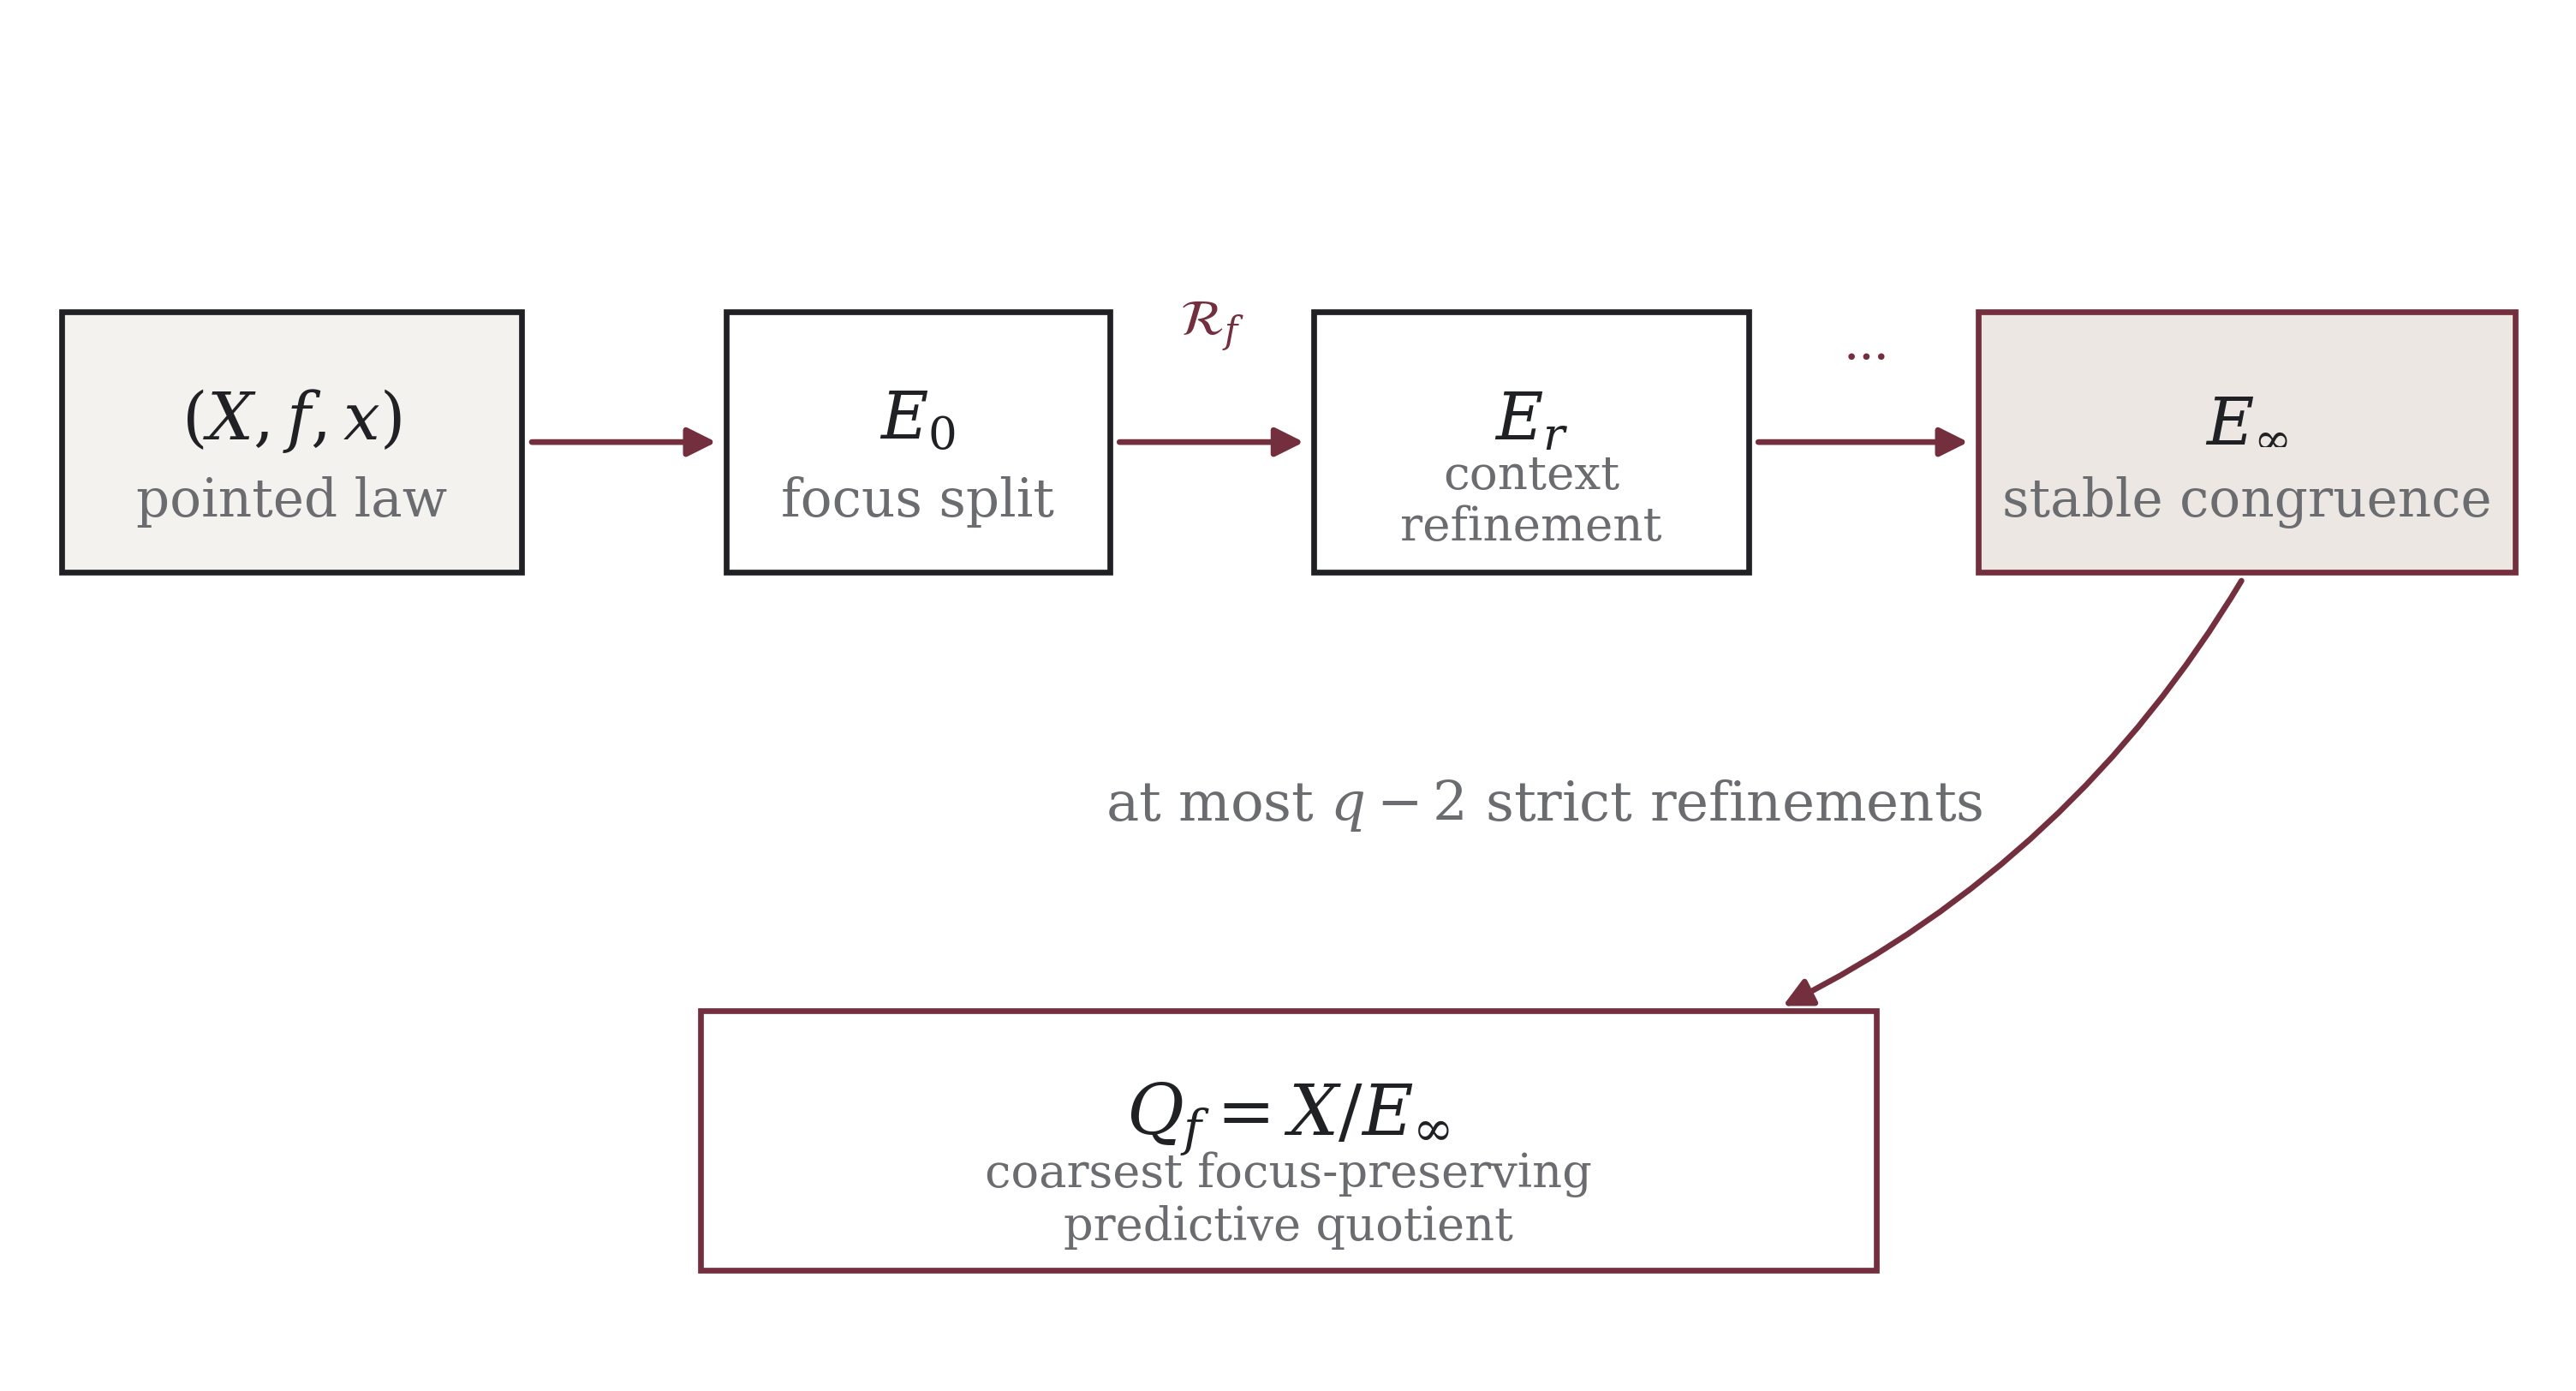
\includegraphics[width=6.12in,height=3.30415in]{figures/rId62.png}

Figure 3. Interaction-generated predictive quotient. Repeated refinement
separates only pairs distinguished by a finite continuation relative to
the retained focus. The stable quotient carries the induced law.

At round \(r\), the generated state is the partition \(E_{r}\), not its
block count. A scalar report may be taken only afterward:

\[k_{r} = \left| X/E_{r} \right| - 1.\]

For the sharp family this shadow is \((1,2,\ldots,q - 1)\). The ordering
is logical dependence under repeated interaction, not physical time. If
\(Q_{f}\) has \(s\) resultants, the corresponding \(P_{1}\) report may
be indexed \(P_{s - 1}\). Both \(k_{r}\) and the perspective index are
read from the closed construction; neither was an input.

\emph{Finite audit.} Every one of the \(3^{3^{2}} = 19,683\)
binary-input laws on a ternary carrier was checked at all three foci,
giving \(59,049\) pointed laws. The audit covered monotonicity,
stabilisation, congruence, the universal property, quotient
reconstruction, cyclic-renaming equivariance, and canonical signatures.

\begin{longtable}[]{@{}
  >{\raggedright\arraybackslash}p{(\columnwidth - 2\tabcolsep) * \real{0.5000}}
  >{\raggedright\arraybackslash}p{(\columnwidth - 2\tabcolsep) * \real{0.5000}}@{}}
\toprule\noalign{}
\begin{minipage}[b]{\linewidth}\raggedright
\textbf{Generated quotient}
\end{minipage} & \begin{minipage}[b]{\linewidth}\raggedright
\textbf{Pointed laws}
\end{minipage} \\
\midrule\noalign{}
\endhead
\bottomrule\noalign{}
\endlastfoot
2 resultants (\(P_{1}\) report) & 3,825 \\
3 resultants (\(P_{2}\) report) & 55,224 \\
Total & 59,049 \\
\end{longtable}

These produce 9,238 label-free predictive isomorphism classes. The
iterative and all-finite-continuation definitions agree in 113 complete
small-law comparisons; all 486 unary ternary pointed permutation cases
are equivariant. The delayed-focus depth formula was also checked for
carrier sizes 2 through 10. These computations audit the theorems; they
do not replace their proofs.

\subsection{Comparing perspectives through a common
source}

Cross-perspective comparison requires a common source. Appending
coordinates to a \(P_{1}\) carrier and declaring \(X \times Q\) a new
perspective is not neutral: the product already contains a deterministic
projection to \(X\), so incomparable descriptions have been ruled out by
construction.

\subsubsection{Future-complete source
quotients}

\emph{Conditional source calculus.} Let \(M\) be a finite family of
source effects closed under declared primitive continuations, and let
\(O_{\theta}\) be a retained observation. Define

\[m\theta n\quad \Leftrightarrow \quad O_{\theta}(wm) = O_{\theta}(wn)\text{ for every finite primitive word }w.\]

The perspective \(P_{\theta} = M/\theta\) inherits every primitive
continuation. The effect family and its primitive actions are declared;
complete future behaviour determines the quotient.

\begin{quote}
\textbf{Theorem CS-1 (translation criterion).} For two such equivalences
\(\theta\) and \(\phi\), a deterministic common-source translation
\end{quote}

\[\lbrack m\rbrack_{\theta} \mapsto \lbrack m\rbrack_{\phi}\]

exists if and only if \(\theta\) refines \(\phi\). When it exists it is
unique and commutes with every primitive continuation.

\emph{Proof.} The displayed assignment is well-defined exactly when
\(m\theta n\) implies \(m\phi n\). Commutation follows because both
quotient actions descend from the same source action. \(\ensuremath{\square}\)

If neither equivalence refines the other, the framework does not invent
a function. It retains the exact same-effect relation

\[\Gamma_{\theta\phi} = \{\left( \lbrack m\rbrack_{\theta},\lbrack m\rbrack_{\phi} \right):m \in M\}.\]

The relation may be one-to-many in both directions. It is exactly the
alignment supported by the common source.

The joint perspective is the common refinement

\[m\theta \land \phi n\quad \Leftrightarrow \quad m\theta n\text{ and }m\phi n.\]

\begin{quote}
\textbf{Theorem CS-2 (strict pairwise creation).} For finite \(M\),
\end{quote}

\[\theta\text{ and }\phi\text{ are incomparable}\quad \Leftrightarrow \quad\left| P_{\theta \land \phi} \right| > \max\left( \left| P_{\theta} \right|,\left| P_{\phi} \right| \right).\]

\emph{Proof.} If the equivalences are incomparable, each separates a
pair merged by the other, so their common refinement strictly splits a
class of each. If one refines the other, their meet is the finer
equivalence and cannot be larger. \(\ensuremath{\square}\)

The common refinement gives a precise meaning to \textbf{joint
organisation}. It combines the two distinction families and, when they
are incomparable, is finer than either marginal quotient. It does not
manufacture a pairwise distinction absent from both: if both \(\theta\)
and \(\phi\) identify two source effects, so does \(\theta \land \phi\).
The gain lies in retaining the two inherited families simultaneously,
not in altering the source.

Figure 4 displays the three comparison objects supplied by the same
source: a direct map under refinement, a relation for incomparable
quotients, and their least joint refinement.

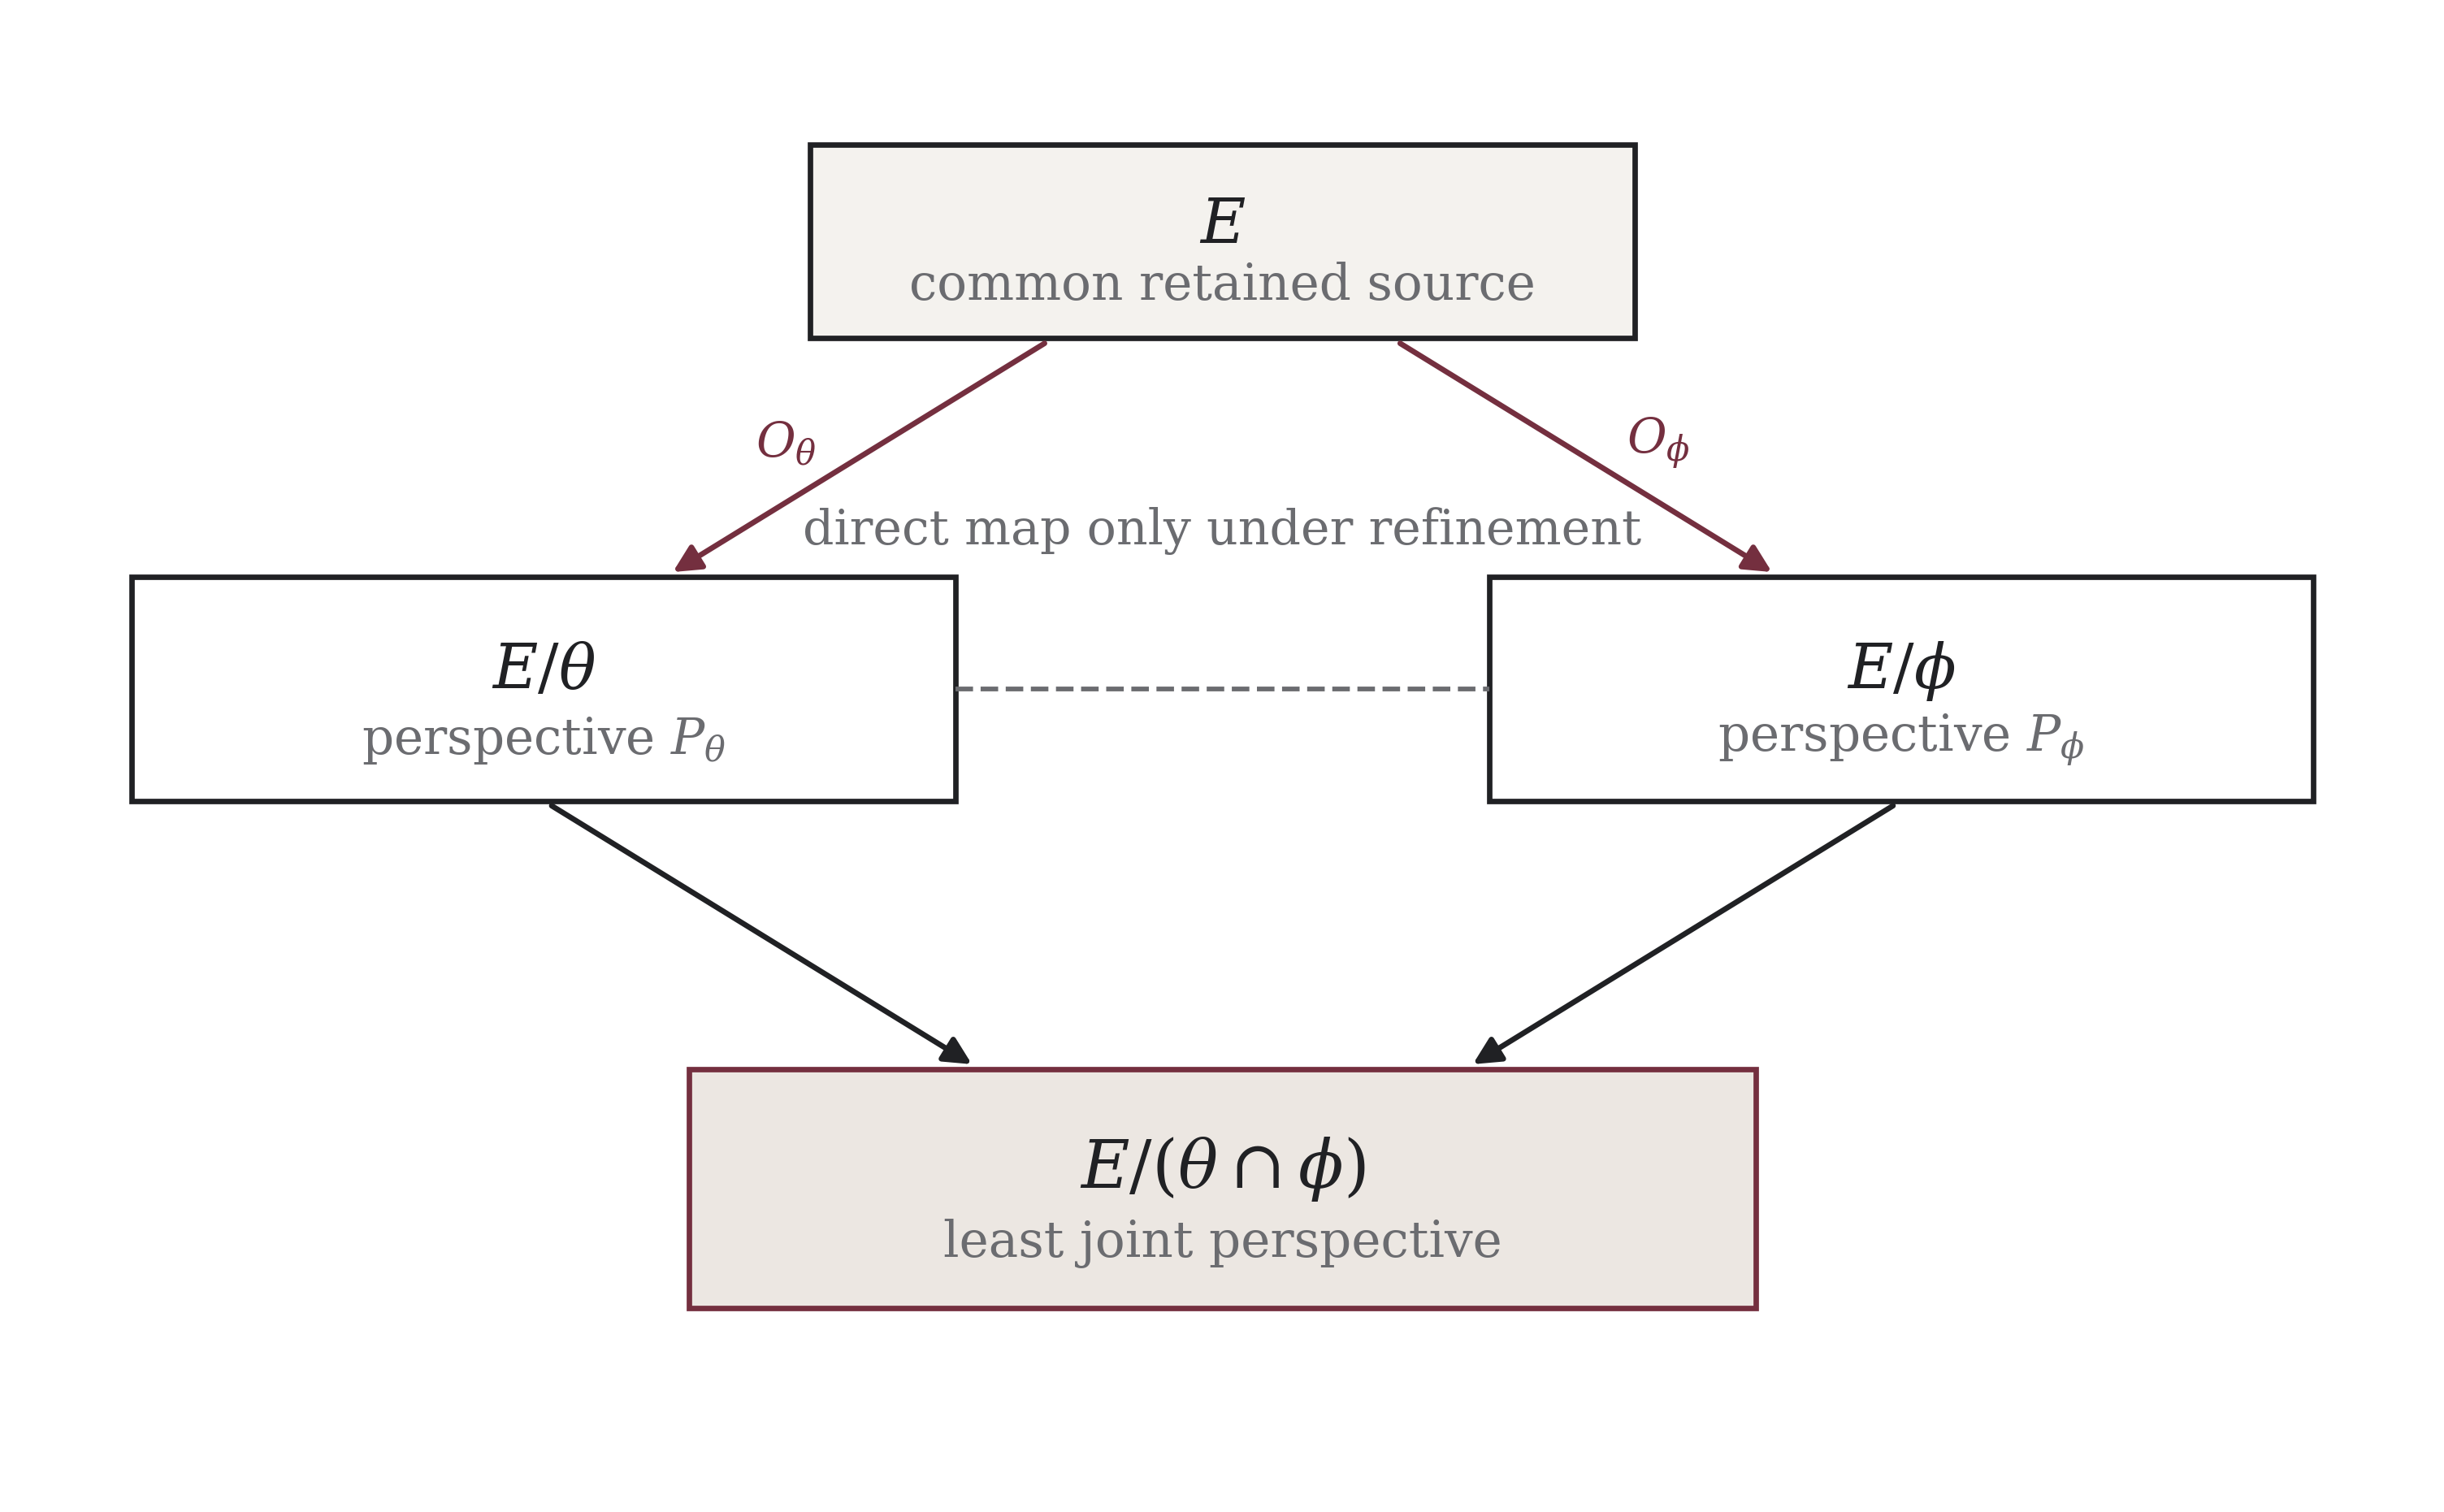
\includegraphics[width=6.12in,height=3.78634in]{figures/rId67.png}

Figure 4. Common-source comparison. Refinement licenses a deterministic
translation. Incomparable quotients retain a source-induced relation and
meet in a strictly finer joint quotient.

\emph{Finite audit.} Across the 1,555 canonical source rules in the
two-transformation census, the comparison produced 774 equivalent
perspective pairs, 3,840 proper one-way pairs, and 51 incomparable
pairs. A rule code such as \texttt{0012\textbar{}1130} lists, on each
side of \texttt{\textbar{}}, the images of \(0,\ldots,n - 1\) under one
of the two generators. Strict joint growth occurred for all and only the
51 incomparable pairs. Three sources produced a joint calculus larger
than each of three audited marginals:

\begin{longtable}[]{@{}
  >{\raggedright\arraybackslash}p{(\columnwidth - 10\tabcolsep) * \real{0.1667}}
  >{\raggedright\arraybackslash}p{(\columnwidth - 10\tabcolsep) * \real{0.1667}}
  >{\raggedright\arraybackslash}p{(\columnwidth - 10\tabcolsep) * \real{0.1667}}
  >{\raggedright\arraybackslash}p{(\columnwidth - 10\tabcolsep) * \real{0.1667}}
  >{\raggedright\arraybackslash}p{(\columnwidth - 10\tabcolsep) * \real{0.1667}}
  >{\raggedright\arraybackslash}p{(\columnwidth - 10\tabcolsep) * \real{0.1667}}@{}}
\toprule\noalign{}
\begin{minipage}[b]{\linewidth}\raggedright
\textbf{Source rule}
\end{minipage} & \begin{minipage}[b]{\linewidth}\raggedright
\textbf{Source effects}
\end{minipage} & \begin{minipage}[b]{\linewidth}\raggedright
\textbf{Kernel}
\end{minipage} & \begin{minipage}[b]{\linewidth}\raggedright
\textbf{Reunion}
\end{minipage} & \begin{minipage}[b]{\linewidth}\raggedright
\textbf{Ideal}
\end{minipage} & \begin{minipage}[b]{\linewidth}\raggedright
\textbf{Joint}
\end{minipage} \\
\midrule\noalign{}
\endhead
\bottomrule\noalign{}
\endlastfoot
\texttt{0012\textbar{}1130} & 13 & 10 & 1 & 8 & 12 \\
\texttt{0012\textbar{}1220} & 14 & 10 & 1 & 10 & 12 \\
\texttt{0013\textbar{}1321} & 16 & 12 & 1 & 11 & 14 \\
\end{longtable}

Allowing each joint calculus to act as the next source produced closed
interaction laws: the first two stabilized as 12-state laws, while the
third passed from 14 states to a fixed 11-state law.

\emph{Finite underdetermination.} Among 376 distinct complete rooted
first-perspective laws, 246 admitted multiple compatible source systems.
In 20 of those cases the other generated perspective laws differed; in
three, even the presence of strict creation differed. These finite pairs
refute unique completion within the declared constructor. A complete
first-perspective law does not, in this census, select a unique
compatible higher-perspective law. The warranted continuation is
therefore the full compatible family; selecting the member nearest a
desired target would import a new assumption.

Chu, sheaf, and institution formalisms each retain relations or contexts
that need not collapse to a single global map (Pratt 1995; Abramsky and
Brandenburger 2011; Goguen and Burstall 1992). The present criterion is
more specific: both views are first closed against one finite source
action, after which refinement decides whether the supported comparison
is functional, relational, or a joint quotient.

\subsection{A target-free binary distinction
game}

The preceding constructions begin with effects or laws. This game begins
one step earlier. After the first \(P_{1}\) distinction, any current
resultant may distinguish into two retained resultants, and the rule may
be applied again. There is no target phenomenon and no global update
schedule.

\subsubsection{Complete transition
family}

\emph{Declared constructor.} Binary continuation is the defining
\(P_{1}\) move. The address marks \(0\) and \(1\) prevent accidental
identification of occurrences; the transition itself never reads them.

A finite record \(E\) is a finite prefix-closed set of binary addresses
containing the root \(\epsilon\), the first already-present distinction.
Its current undistinguished resultants are

\[B(E) = \{ w:(\exists v \in E)(w = v0 \vee w = v1),\ w \notin E\}.\]

The next step retains the complete successor family

\[\mathcal{D}(E) = \{\left( x,E \cup \{ x\} \right):x \in B(E)\}.\]

The ordered pair retains which existing occurrence was continued and the
resulting complete record.

Let \(\sigma\) denote a prefix-preserving automorphism of the rooted
binary address tree generated by local exchanges of the marks \(0\) and
\(1\). It acts componentwise on addresses, records, and transitions:

\[\sigma(x,E): = (\sigma x,\sigma E).\]

\begin{quote}
\textbf{Theorem TF (generated continuation laws).} The transition family
satisfies all of the following.
\end{quote}

\begin{enumerate}
\def\labelenumi{\arabic{enumi}.}
\item
  \textbf{Local replacement.} For every \(x \in B(E)\),
\end{enumerate}

\[B\left( E \cup \{ x\} \right) = \{ y \in B(E):y \neq x\} \cup \{ x0,x1\}.\]

\begin{enumerate}
\def\labelenumi{\arabic{enumi}.}
\setcounter{enumi}{1}
\item
  \textbf{Inert-name equivariance.} Any recursively applied exchange of
  the address marks bijects the complete transition family:
\end{enumerate}

\[\sigma\left( \mathcal{D}(E) \right) = \mathcal{D}(\sigma E).\]

\begin{enumerate}
\def\labelenumi{\arabic{enumi}.}
\setcounter{enumi}{2}
\item
  \textbf{Commutation at separate current occurrences.} If \(x \neq y\)
  lie in \(B(E)\), then
\end{enumerate}

\[\left( E \cup \{ x\} \right) \cup \{ y\} = \left( E \cup \{ y\} \right) \cup \{ x\}.\]

\begin{enumerate}
\def\labelenumi{\arabic{enumi}.}
\setcounter{enumi}{3}
\item
  \textbf{Ancestry-only history restriction.} Finite resultant records
  are exactly the finite prefix-closed address sets containing
  \(\epsilon\). Legal histories of a fixed record are exactly its linear
  extensions under ancestry. Any two differ by exchanges of adjacent
  unrelated occurrences.
\item
  \textbf{Common core and common completion.} If \(E\) and \(F\) are
  legal, then \(E \cap F\) and \(E \cup F\) are legal. They obey
  absorption and distributivity as set identities.
\item
  \textbf{Unique continuation factorisation.} Every extension
  \(F \supseteq E\) decomposes uniquely into one local continuation
  below each \(x \in B(E)\):
\end{enumerate}

\[F_{x} = \{ u:xu \in F\},\]

\begin{itemize}
\item
  where \(F_{x} = \varnothing\) records no continuation below \(x\).
  Then
\end{itemize}

\[F = E \cup \bigcup_{x \in B(E)}xF_{x}.\]

\begin{enumerate}
\def\labelenumi{\arabic{enumi}.}
\setcounter{enumi}{6}
\item
  \textbf{No finite terminal record.} \(B(E) \neq \varnothing\) for
  every finite \(E\).
\end{enumerate}

\emph{Proof.} If \(x \in B(E)\), inserting \(x\) removes that boundary
address and introduces exactly its two children, which proves local
replacement. A prefix-preserving tree automorphism sends boundary
addresses to boundary addresses and commutes with adjoining a node;
applying this pointwise gives inert-name equivariance. If \(x\) and
\(y\) are distinct boundary addresses, neither is a prefix of the other.
Inserting one therefore leaves the other on the boundary, and both
update orders produce \(E \cup \{ x,y\}\).

Every reachable record contains \(\epsilon\) and is prefix-closed
because an address can be inserted only after all of its proper
prefixes. Conversely, for a finite prefix-closed set \(F\) containing
\(\epsilon\), order all other elements of \(F\) by nondecreasing length.
Each address is on the current boundary when selected, so this order
constructs \(F\). More generally, a construction history for fixed \(F\)
is legal exactly when every prefix precedes its descendants---precisely
when it is a linear extension of the ancestry order. Any two linear
extensions of a finite poset are connected by swaps of adjacent
incomparable elements: repeatedly move the next element of one extension
leftward through elements that cannot precede it in the other.

Union and intersection preserve prefix closure and the root. For an
extension \(F \supseteq E\), every new address has a unique longest
prefix \(x \in B(E)\); the boundary is prefix-incomparable, so the
resulting sets \(xF_{x}\) are disjoint and collectively contain
precisely the elements of \(F\) not already in \(E\). This proves
existence and uniqueness of the factorisation. Finally, take an address
of maximal length in finite \(E\). Neither child can lie in \(E\), so
both are in \(B(E)\) and the boundary is nonempty. \(\ensuremath{\square}\)

These relations can subsequently be identified with familiar structures.
Legal records form a distributive lattice under union and intersection;
a fixed record carries an ancestry poset; complete records have rooted
full binary-tree shapes; independent local continuations give a
recursive species decomposition (Birkhoff 1967; Stanley 2015; Bergeron,
Labelle, and Leroux 1998). These identifications describe the result;
they do not define the transition.

\subsubsection{Enumeration after
closure}

Counting is applied only after the transition has been fixed. If
\(A_{n}\) denotes the number of complete identity records with \(n\)
distinguished occurrences and \(A_{0} = 1\) denotes an empty local
continuation, unique root factorisation gives

\[A_{n} = \sum_{i + j = n - 1}^{}A_{i}A_{j},\quad\quad A_{n} = \frac{1}{n + 1}\binom{2n}{n}.\]

The local replacement identity implies that every \(n\)-occurrence
record has \(n + 1\) current resultants. The total number of legal
histories at level \(n\) is consequently \(2 \cdot 3\cdots n = n!\). For
a fixed record \(E\), let \(s_{E}(v)\) be the number of distinguished
occurrences at or below a non-root occurrence \(v\). Its history
multiplicity is

\[H(E) = \frac{\left( |E| - 1 \right)!}{\prod_{v \in E,\ v \neq \epsilon}^{}s_{E}(v)}.\]

The proof interleaves the independent histories below the two root
resultants and proceeds recursively.

\begin{longtable}[]{@{}
  >{\raggedright\arraybackslash}p{(\columnwidth - 6\tabcolsep) * \real{0.2500}}
  >{\raggedright\arraybackslash}p{(\columnwidth - 6\tabcolsep) * \real{0.2500}}
  >{\raggedright\arraybackslash}p{(\columnwidth - 6\tabcolsep) * \real{0.2500}}
  >{\raggedright\arraybackslash}p{(\columnwidth - 6\tabcolsep) * \real{0.2500}}@{}}
\toprule\noalign{}
\begin{minipage}[b]{\linewidth}\raggedright
\textbf{Distinguished occurrences}
\end{minipage} & \begin{minipage}[b]{\linewidth}\raggedright
\textbf{Complete records}
\end{minipage} & \begin{minipage}[b]{\linewidth}\raggedright
\textbf{Complete legal histories}
\end{minipage} & \begin{minipage}[b]{\linewidth}\raggedright
\textbf{Current resultants per record}
\end{minipage} \\
\midrule\noalign{}
\endhead
\bottomrule\noalign{}
\endlastfoot
1 & 1 & 1 & 2 \\
2 & 2 & 2 & 3 \\
3 & 5 & 6 & 4 \\
4 & 14 & 24 & 5 \\
5 & 42 & 120 & 6 \\
6 & 132 & 720 & 7 \\
7 & 429 & 5,040 & 8 \\
8 & 1,430 & 40,320 & 9 \\
\end{longtable}

The finite audit covered 19,631 configuration/boundary identities,
17,576 recursive name exchanges, 67,071 separate-resultant diamonds,
390,625 union/intersection pairs, 6,968 continuation decompositions, and
the history formula for all 2,055 records through level eight. No
counterexample was found. The all-finite claims rest on the proofs
above, not on the bounded audit.

Unlike a cellular automaton, the game has no ambient lattice,
neighbourhood, synchronous clock, or selected update table (Wolfram
1984). Its object is an extensible genealogy together with every legal
local continuation. The resulting lattice, factorisation, and counting
laws are consequences of that transition rather than criteria imposed
upon it.

\subsection{Projection towers and erased
distinctions}

A complete record admits several autonomous projections. Studying them
together separates closure from mere loss of information.

\subsubsection{Four continuation-closed
views}

\emph{Declared projections.} Let \(H_{d}\) be the complete set of
explicit histories after \(d\) distinctions, and consider the tower

\[H_{d}\overset{\alpha_{d}}{\rightarrow}O_{d}\overset{\beta_{d}}{\rightarrow}U_{d}\overset{\gamma_{d}}{\rightarrow}C_{d}.\]

Here \(O_{d}\) forgets the temporal trace but retains the ordered
current form; \(U_{d}\) also forgets every temporary left/right order;
and \(C_{d}\) keeps only the number of available occurrences. None is
designated as the true view.

For an ordered form \(T\), let \(d_{v}\) be the number of internal
occurrences in the subform rooted at \(v\). For an order-free form
\(T\), assign each internal occurrence a factor \(w_{v} = 1\) when its
two subforms coincide and \(w_{v} = 2\) when they differ, and define

\[e(T) = \prod_{v}^{}w_{v}.\]

Then the exact fibre sizes are

\[\left| \alpha_{d}^{- 1}(T) \right| = \frac{d!}{\prod_{v}^{}d_{v}},\quad\quad\left| \beta_{d}^{- 1}(T) \right| = e(T),\quad\quad\left| \left( \beta_{d} \circ \alpha_{d} \right)^{- 1}(T) \right| = \frac{d!e(T)}{\prod_{v}^{}d_{v}}.\]

The first formula follows by recursively interleaving subtree histories;
the second assigns two orientations to every unequal pair of subforms
and one to an equal pair. Since every level-\(d\) form has \(d + 1\)
available occurrences, \(C_{d}\) has one class and its history fibre has
size \(d!\).

A view is \textbf{continuation-closed} if the multiset of next-view
results from all current distinctions depends only on the view-class and
not on its representative.

\begin{quote}
\textbf{Theorem PT (projection closure and counting barrier).} Every
view \(H,O,U,C\) is continuation-closed. Continued distinction within
the count-only view \(C\), however, cannot regenerate any arrangement,
orientation, or history distinction erased by \(\gamma\beta\alpha\).
\end{quote}

\emph{Proof.} In \(H_{d}\) the complete successor multiset is part of
the definition, so closure is immediate. The projection \(\alpha_{d}\)
erases only the order in which already recorded distinctions were made;
it leaves the current ordered form and its available addresses
unchanged. Hence representatives of one \(O_{d}\)-class have identical
\(O_{d + 1}\) successor multisets. Two ordered representatives of one
\(U_{d}\)-class differ by finitely many local left/right exchanges. Each
exchange bijects their available addresses, commutes with a continuation
at the corresponding address, and yields order-free-isomorphic
successors. Thus their projected successor multisets agree. Finally,
every level-\(d\) record has exactly \(d + 1\) available current
occurrences, and every continuation enters the sole class of
\(C_{d + 1}\). The count successor multiset therefore depends only on
\(d\).

For the barrier, induction on continuation length shows that every
response generated from a \(C_{d}\)-class remains inside one count class
at each later level. An autonomous continuation on \(C\) therefore has
no response that separates two representatives already merged by
\(\gamma\beta\alpha\). Arrangement, orientation, and history
distinctions cannot be regenerated inside the count-only quotient. \(\ensuremath{\square}\)

This is \textbf{stable blindness} in a concrete tower. The erased
distinctions remain available in \(H_{d}\), \(O_{d}\), and \(U_{d}\),
but they are absent from \(C_{d}\) and cannot be recreated by its
autonomous continuation. A scalar count can therefore support a simpler
law while retaining strictly less source structure.

Figure 5 makes the direction of information loss explicit: every forward
projection is continuation-closed, but there is no closed inverse.

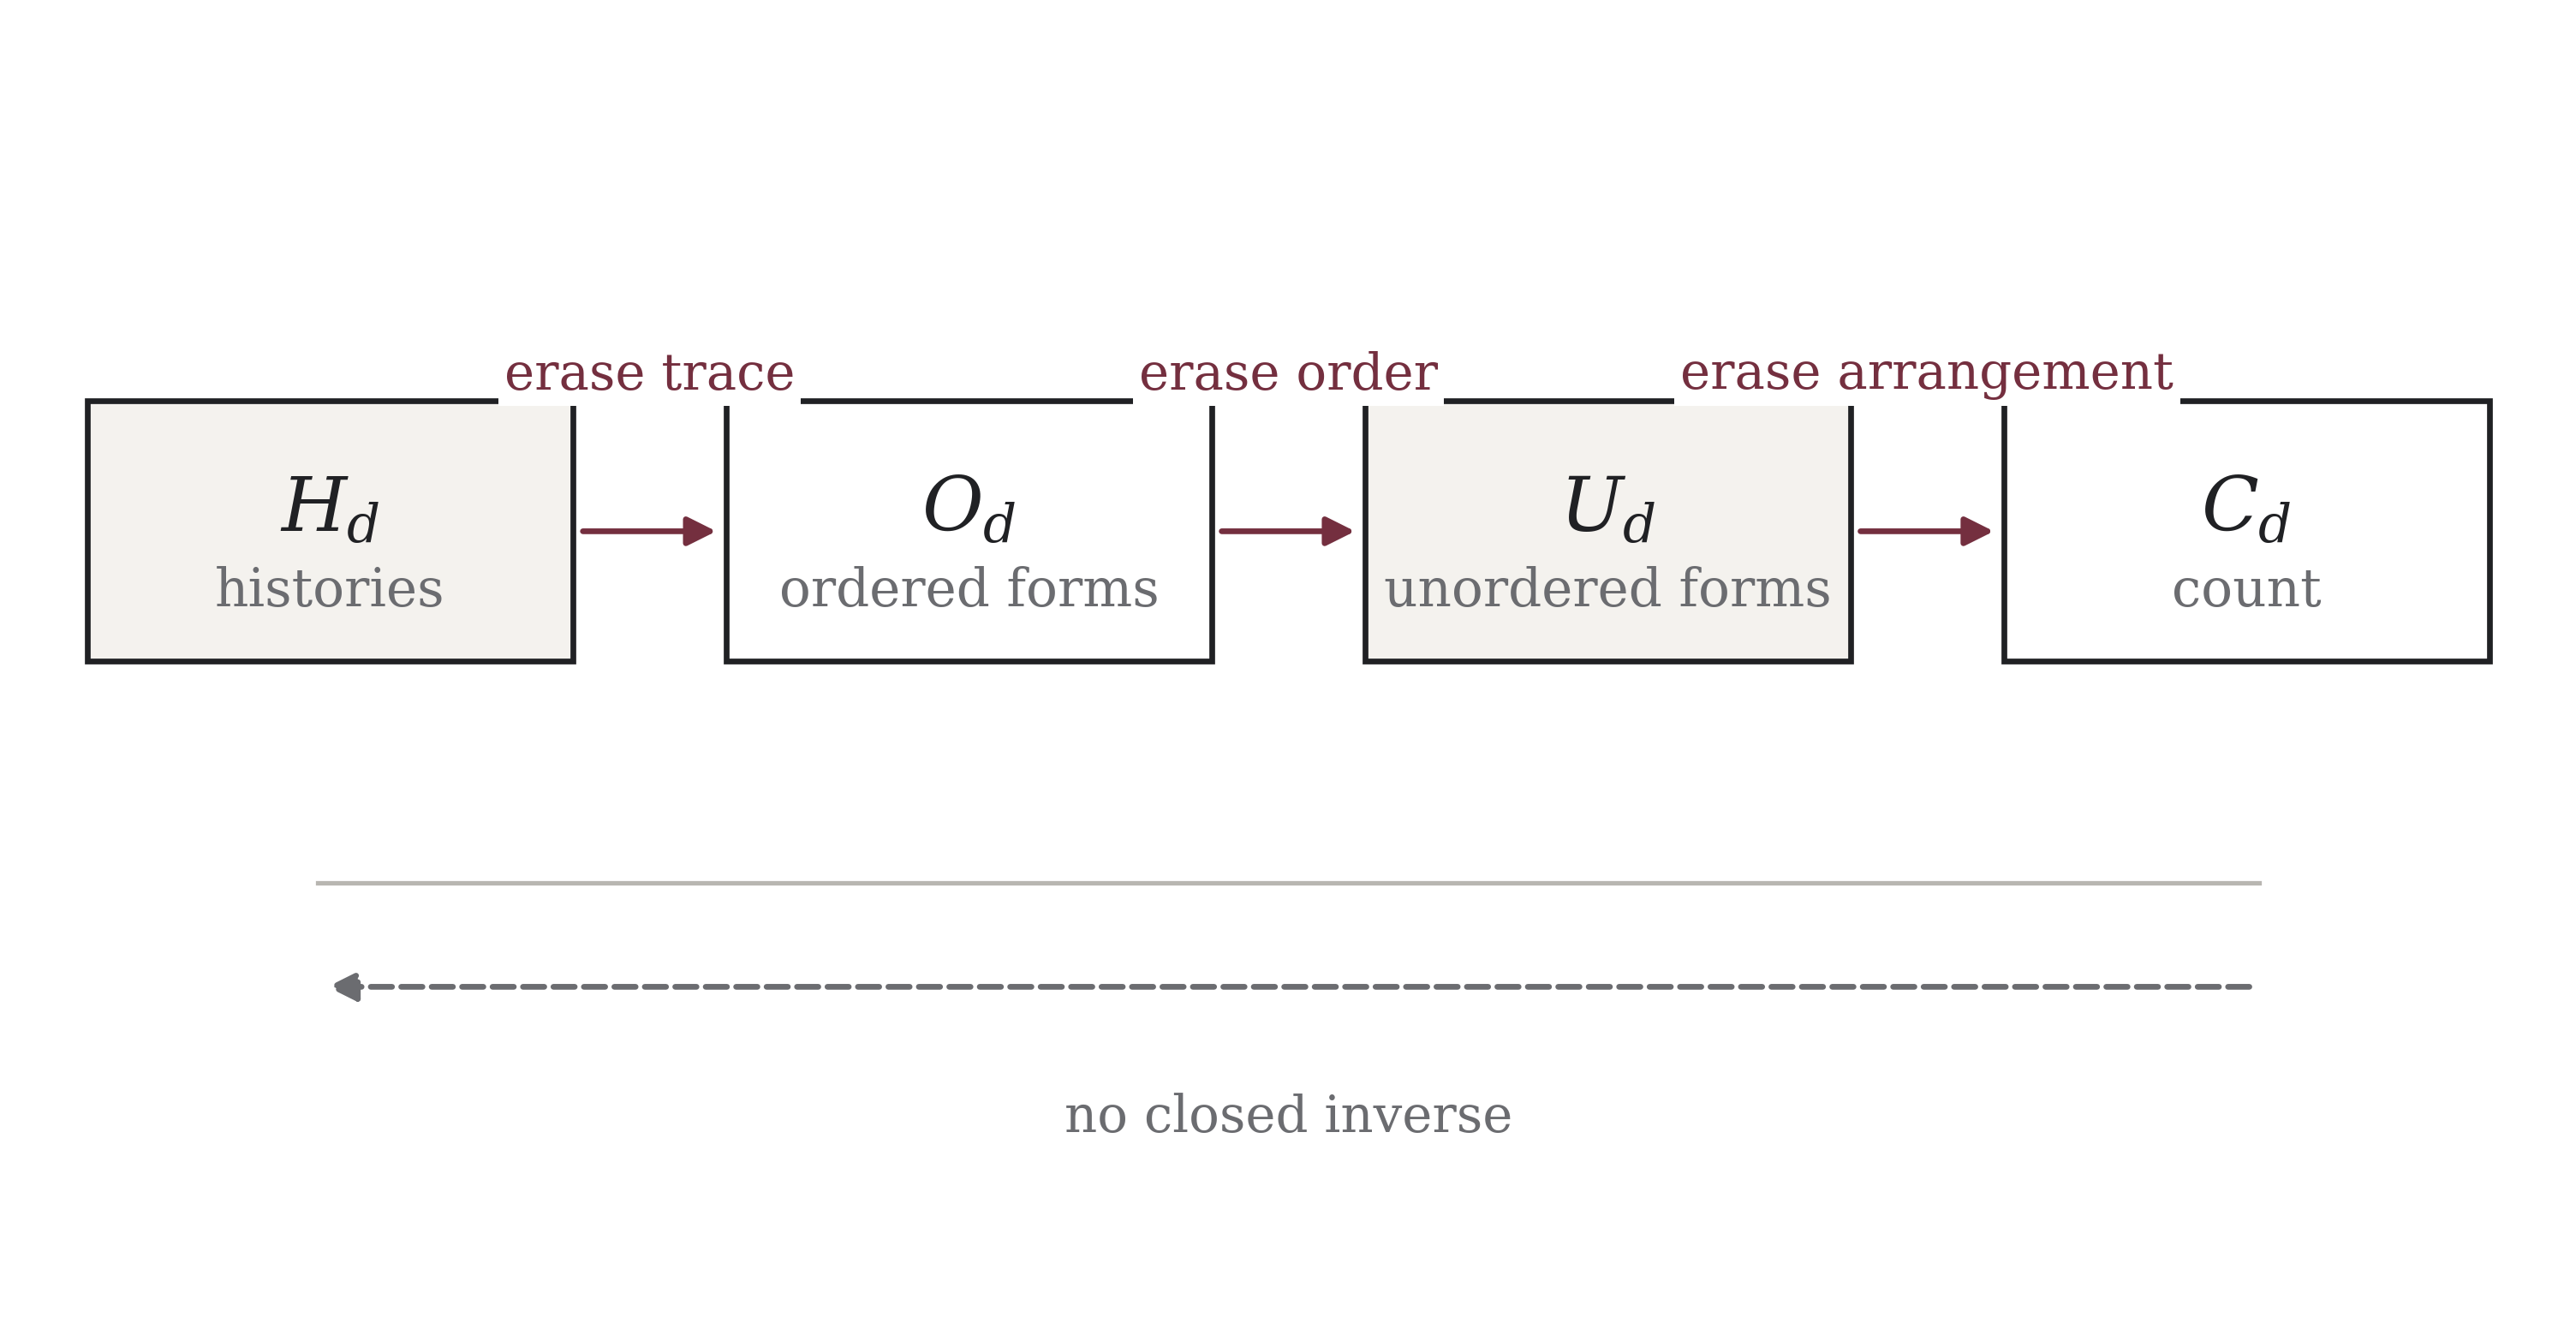
\includegraphics[width=6.12in,height=3.14342in]{figures/rId75.png}

Figure 5. Projection tower. Each quotient supports an autonomous
continuation, but no continuation within a quotient recovers
distinctions erased by the preceding projection.

\subsubsection{\texorpdfstring{4.5.2 Complete partitions before scalar
\(k\)}{4.5.2 Complete partitions before scalar k}}

Let \(\Pi\) and \(\Sigma\) be continuation-closed partitions of the same
forms. Retaining every distinction made by either produces their common
refinement

\[x \sim_{\Pi \vee \Sigma}y\quad \Leftrightarrow \quad x \sim_{\Pi}y\text{ and }x \sim_{\Sigma}y.\]

Although the symbol \(\vee\) is conventional here, the operation is the
intersection of equivalence relations: the coarsest partition refining
both. It is forced by complete retention and is commutative,
associative, and idempotent.

Let \(S\) and \(T\) be finite source and target sets, and let
\(A:S \times T \rightarrow \mathbb{N}\) record continuation
multiplicity. For a partition \(\Pi\) of \(T\), define the source
partition \(F_{A}(\Pi)\) by

\[s \sim_{F_{A}(\Pi)}s\prime\quad \Leftrightarrow \quad\sum_{t \in B}^{}A(s,t) = \sum_{t \in B}^{}A(s\prime,t)\text{ for every block }B \in \Pi.\]

\begin{quote}
\textbf{Theorem PI (partition interaction).} If \(\Pi\) refines
\(\Sigma\), then \(F_{A}(\Pi)\) refines \(F_{A}(\Sigma)\). Moreover,
\end{quote}

\[F_{A}(\Pi \vee \Sigma)\text{ refines }F_{A}(\Pi) \vee F_{A}(\Sigma).\]

The refinement may be strict.

\emph{Proof.} Each \(\Sigma\)-block is a union of \(\Pi\)-blocks, so
equality of all fine-block counts implies equality of their coarse sums.
Joint block counts determine both marginal block-count vectors, proving
the second refinement. Marginal vectors need not determine their joint
table, so the converse can fail. \(\ensuremath{\square}\)

The strict difference defines the interaction-only distinction relation
\(\mathcal{I}_{A}(\Pi,\Sigma)\): it consists of source pairs equivalent
under \(F_{A}(\Pi) \vee F_{A}(\Sigma)\) but inequivalent under
\(F_{A}(\Pi \vee \Sigma)\).

It contains source pairs that neither marginal pullback separates but
the complete joint pullback does. A horizon-eight witness has six
classes under separate pullback-and-combination and seven under joint
combination-then-pullback. Its two level-six forms

\[\left( \left( \left( (..). \right)(..) \right)(..) \right)\quad\text{and}\quad\left( \left( (..)(..) \right)\left( (..). \right) \right)\]

have identical marginal signatures but different joint signatures.

The scalar barrier is stronger than a loss of labels. At level 5,
retained partitions with class counts \(2\) and \(3\) can interact to
produce either \(3\) or \(4\) classes. Consequently no function \(f\)
satisfies

\[|\Pi \vee \Sigma| = f\left( |\Pi|,|\Sigma| \right)\]

even in this finite generated family. Before a further projection is
specified, the complete objects are the partitions themselves,

\[K_{P} = \Pi_{P},\quad\quad I(P,Q) = \mathcal{I}_{A}\left( \Pi_{P},\Pi_{Q} \right),\]

not their cardinalities. A numerical \(k\) is a downstream shadow.
Information measures based on scalar costs over a fixed alphabet remain
valid in their intended domains (Hartley 1928; Shannon 1948; Cover and
Thomas 2006); they begin after the distinctions kept explicit here have
already been fixed.

\subsection{Conditional laboratory: an open finite-rule
census}

The target-free game isolates the consequences of one binary
continuation. A separate laboratory admits richer source structure in
order to study the closed laws and perspectives it generates. Its
findings are conditional on that choice of source.

\subsubsection{Declared branch}

Choose a finite carrier \(X = \{ 0,\ldots,n - 1\}\), with
\(n \in \{ 2,3,4\}\); two arbitrary total transformations
\(a,b:X \rightarrow X\); identity; and ordinary composition. Products
are written \(gm: = g \circ m\), so \(m\) acts first. Retain every
unordered primitive pair with repetition, quotienting only by carrier
relabelling and exchange of primitive names. These are declared
laboratory conditions, not consequences of the sole distinction rule.
Algebraic claims below hold for every finite system satisfying their
displayed hypotheses. Counts and classifications are exhaustive only at
the stated carrier sizes.

The exhaustive finite census begins with the following source counts.

\begin{longtable}[]{@{}
  >{\raggedright\arraybackslash}p{(\columnwidth - 6\tabcolsep) * \real{0.2500}}
  >{\raggedright\arraybackslash}p{(\columnwidth - 6\tabcolsep) * \real{0.2500}}
  >{\raggedright\arraybackslash}p{(\columnwidth - 6\tabcolsep) * \real{0.2500}}
  >{\raggedright\arraybackslash}p{(\columnwidth - 6\tabcolsep) * \real{0.2500}}@{}}
\toprule\noalign{}
\begin{minipage}[b]{\linewidth}\raggedright
\textbf{Carrier size}
\end{minipage} & \begin{minipage}[b]{\linewidth}\raggedright
\textbf{Raw primitive pairs}
\end{minipage} & \begin{minipage}[b]{\linewidth}\raggedright
\textbf{Canonical systems}
\end{minipage} & \begin{minipage}[b]{\linewidth}\raggedright
\textbf{Distinct invariant profiles}
\end{minipage} \\
\midrule\noalign{}
\endhead
\bottomrule\noalign{}
\endlastfoot
2 & 10 & 7 & 6 \\
3 & 378 & 74 & 67 \\
4 & 32,896 & 1,474 & 1,175 \\
\end{longtable}

Within this census, two primitive transformations generate up to 176
effective transformations.

\begin{quote}
\textbf{Proposition OR-1 (ideal and rank order).} In every generated
transformation monoid \(M\), composition induces a one-way preorder. For
the two-sided ideal \(I(m) = MmM\) and every \(g \in M\),
\end{quote}

\[rank(gm) \leq rank(m),\quad\quad I(gm) \subseteq I(m).\]

\emph{Proof.} The image of \(gm\) is the image under \(g\) of the image
of \(m\), so it has at most \(rank(m)\) elements. Moreover,

\[I(gm) = MgmM \subseteq MmM = I(m),\]

because \(Mg \subseteq M\). Repeating the argument after any further
left composition proves that a strict ideal descent cannot later be
reversed. \(\ensuremath{\square}\)

Further composition cannot reverse strict ideal descent, although
recurrence may occur within a level. This is an internal order and
carries no automatic interpretation as time, entropy, causality, or
knowledge.

\subsubsection{Quotients and predictive
closure}

Among the 1,474 four-state systems, 1,171 have proper nontrivial
congruence quotients, 529 have incomparable quotient pairs, and 270
exhibit distributed effect recovery: no proper quotient is faithful
alone, while the retained quotient family is jointly faithful. For rule
\texttt{1002\textbar{}2210}, two incomparable three-block quotients each
distinguish 7 of 14 generated effects and together distinguish all 14.

\begin{quote}
\textbf{Proposition OR-2 (kernel and predictor order).} Each generated
effect \(m\) has a kernel \(\kappa_{m}\), where \(x\kappa_{m}y\) iff
\(m(x) = m(y)\). Along \(m \mapsto g \circ m\), kernels can only
coarsen. If \(K\) is the number of current-kernel classes, \(Q\) the
number of classes under
\end{quote}

\[m \equiv_{\kappa}n\quad \Leftrightarrow \quad\ker(xm) = \ker(xn)\text{ for every }x \in M,\]

and \(E = |M|\) the number of full effects, then

\[K \leq Q \leq E.\]

\emph{Proof.} If \(m(u) = m(v)\), then
\(g\left( m(u) \right) = g\left( m(v) \right)\), so
\(\kappa_{m} \subseteq \kappa_{gm}\). For the class count, equality of
effects implies \(\equiv_{\kappa}\), while \(m \equiv_{\kappa}n\)
implies \(\ker(m) = \ker(n)\) by taking \(x\) to be the identity. Thus
full-effect equality refines \(\equiv_{\kappa}\), which refines
current-kernel equality, and the displayed inequality follows. \(\ensuremath{\square}\)

The present kernel often fails to determine its successor. Among
four-state systems, 1,446 show strict kernel descent, 811 have
incomparable successor-kernel branches, 995 show kernel-level predictive
failure, and 1,128 reach kernels that are not global congruences.

The equivalence \(\equiv_{\kappa}\) is therefore the predictive
quotient: it retains exactly the distinctions required to determine
every future kernel history.

The four-state systems divide into three predictive regimes:

\begin{longtable}[]{@{}
  >{\raggedright\arraybackslash}p{(\columnwidth - 4\tabcolsep) * \real{0.3333}}
  >{\raggedright\arraybackslash}p{(\columnwidth - 4\tabcolsep) * \real{0.3333}}
  >{\raggedright\arraybackslash}p{(\columnwidth - 4\tabcolsep) * \real{0.3333}}@{}}
\toprule\noalign{}
\begin{minipage}[b]{\linewidth}\raggedright
\textbf{Four-state regime}
\end{minipage} & \begin{minipage}[b]{\linewidth}\raggedright
\textbf{Systems}
\end{minipage} & \begin{minipage}[b]{\linewidth}\raggedright
\textbf{Interpretation inside the branch}
\end{minipage} \\
\midrule\noalign{}
\endhead
\bottomrule\noalign{}
\endlastfoot
\(Q = K\) & 479 & current kernel is already autonomous \\
\(K < Q = E\) & 158 & every full-effect distinction is required \\
\(K < Q < E\) & 837 & a genuine intermediate predictor is forced \\
\end{longtable}

For \texttt{0032\textbar{}2031}, \(K = 12\), \(Q = 137\), and
\(E = 176\): 39 full-effect distinctions are irrelevant to every future
kernel history, but the kernel alone omits distinctions needed to
predict its future.

\begin{quote}
\textbf{Theorem OR-3 (recursive-lift termination).} Treating the
predictor as a transformation system and repeating the construction
gives a finite recursive lift. After the first lift each proper step is
a strict quotient. Up to pointed-monoid isomorphism, every finite
trajectory reaches a fixed point and cannot enter a nontrivial cycle.
\end{quote}

\emph{Proof.} The relation \(\equiv_{\kappa}\) is a two-sided monoid
congruence. If \(m \equiv_{\kappa}n\), then for any \(y \in M\) and
every left context \(x\),

\[\ker(xym) = \ker(xyn),\]

which proves left stability. For right stability, equality of
\(\ker(xm)\) and \(\ker(xn)\) implies equality after pullback by \(y\):

\[\ker\left( (xm)y \right) = y^{- 1}\left( \ker(xm) \right) = y^{- 1}\left( \ker(xn) \right) = \ker\left( (xn)y \right).\]

Hence the predictive classes form the quotient monoid
\(C = M/ \equiv_{\kappa}\). The lifted system is the left-regular action
of \(C\) on itself,
\(\lbrack u\rbrack:\lbrack m\rbrack \mapsto \lbrack um\rbrack\).
Distinct elements induce distinct transformations because their actions
on the identity class differ, so the lifted carrier and its generated
effect monoid both have cardinality \(|C|\). Identifying \(C\) with this
faithful regular representation, every subsequent lift is a quotient of
the preceding finite monoid. A proper lift strictly reduces cardinality;
a nontrivial cycle would require a later increase or a proper quotient
of equal cardinality, both impossible. Finite descent terminates at a
fixed point up to pointed isomorphism. \(\ensuremath{\square}\)

Across all 1,555 canonical systems, 1,523 are fixed after the first
lift, 32 require one further quotient, and all converge to 369 pointed
fixed systems. The largest expansion is
\(4 \rightarrow 137 \rightarrow 137\); the largest second reduction is
\(4 \rightarrow 8 \rightarrow 4 \rightarrow 4\).

\subsubsection{Endogenous futures and irreversible opportunity
loss}

\begin{quote}
\textbf{Proposition OR-4 (future-domain and reunion order).} Let a
finite monoid \(M\) act on \(X\). For \(x \in X\), put \(I_{x} = Mx\).
Every \(g \in M\) satisfies \(I_{gx} \subseteq I_{x}\), and
\(I_{x} = I_{y}\) exactly when \(x\) and \(y\) are mutually reachable.
\end{quote}

\emph{Proof.} Since \(Mg \subseteq M\), we have
\(I_{gx} = M(gx) = (Mg)x \subseteq Mx = I_{x}\). If \(I_{x} = I_{y}\),
then \(x \in I_{y}\) and \(y \in I_{x}\), so each state reaches the
other. Conversely, mutual reachability gives both inclusions between the
generated domains. \(\ensuremath{\square}\)

Across the 369 fixed systems, 11,211 states generate 3,059 distinct
principal domains; 368 systems have strict domain descent, 246 have
incomparable primitive branches, and 29 have multiple minimal terminal
domains.

\textbf{Reunion-capacity monotonicity.} For an unordered pair \(x,y\),
define reunion capacity by three exhaustive cases:

\begin{itemize}
\tightlist
\item
  \(\chi(x,y) = 2\) when some \(u \in M\) satisfies \(u(x) = u(y)\);
\item
  \(\chi(x,y) = 1\) when \(I_{x} \cap I_{y} \neq \varnothing\) but no
  common \(u\) merges the pair;
\item
  \(\chi(x,y) = 0\) when \(I_{x} \cap I_{y} = \varnothing\).
\end{itemize}

Then every generated continuation obeys

\[\chi(gx,gy) \leq \chi(x,y).\]

\emph{Proof.} If the target pair \((gx,gy)\) has a merger \(u\), then
\(ug\) merges \((x,y)\), so capacity \(2\) at the target implies
capacity \(2\) at the source. If \(I_{gx} \cap I_{gy}\) is nonempty, the
domain inclusions already proved give
\(I_{x} \cap I_{y} \neq \varnothing\); thus positive target capacity
implies positive source capacity. These are all three ordered cases,
proving the inequality. \(\ensuremath{\square}\)

Opportunity may therefore be lost but cannot be recovered under a shared
continuation.

The complete census classifies 347,335 unordered distinct pairs: 346,991
are coalescible by a common continuation, 131 overlap only under
different continuations, and 213 have disjoint future domains. It
records 347 strict primitive decreases: 37 of type \(2 \rightarrow 1\),
207 of type \(2 \rightarrow 0\), and 103 of type \(1 \rightarrow 0\).
The monotonicity inequality was independently checked in 31,930,235
pair/effect applications.

For an effect \(m\), the future-profile construction retains
\(\Lambda_{m}(x,y) = \chi\left( m(x),m(y) \right)\) and identifies two
effects exactly when all their future profiles agree.

Present reunion capacity is not always autonomous. Across the 369 fixed
systems, 11,211 effects yield 484 current profiles, while complete
future prediction requires 552 states. Twenty-two systems require hidden
refinement, and four force an intermediate carrier strictly between
present-profile and full-effect descriptions. Recursive future-profile
closure terminates in 22 fixed systems, with no expansion or nontrivial
cycle.

\subsubsection{What the laboratory establishes---and what it
cannot
establish}

The census supplies exact examples of transformation growth,
irreversible ideal and kernel orders, incomparable quotients,
distributed recovery, minimal predictors, recursive closure, distinct
local futures, monotone opportunity loss, and interaction-created
distinctions. It also gives counterexamples to several scalar and
functional simplifications.

The finite carrier, total transformations, composition, identity, and
two-primitive source are laboratory inputs. They are not derived from
\(P_{0}/R\) or from the binary constructor. Kernel depth is not equated
with \(k\), a predictive class with an actual perspective, or ideal
descent with physical time. Exhaustion at \(n \leq 4\) establishes the
census, not a theorem beyond it.

The laboratory separates two questions: what follows from the declared
interaction, and whether that interaction models a named phenomenon.
Only the first is addressed here. Fifty-six automated tests cover all
1,555 canonical systems, 32,926 generated effects, 28,313 ordered
quotient pairs, 20,317 minimised predictive states, 31,930,235
opportunity-loss checks, and an independent reconstruction of every
recorded quotient and profile. These tests assess the calculus and its
implementation; they do not privilege one audited system as a model of
reality.

The falsifiability section records the corresponding counterexamples and
provenance failures. None of the finite representations is asserted to
exhaust the possible perspectives of \(R\).

\section{Prime-source occurrences and the 36-relation frontier}
The elementary identity $p\cdot1=p$ supplies a compact example of the source/report distinction. The two $p$ tokens have equal value but different source and returned-product roles. A value reporter merges them; an occurrence-sensitive reporter retains the relation
\begin{equation}
p_{\rm source}\cdot1_{\rm unit}=p_{\rm return}.
\end{equation}
The reduced triad contains every positive factor relation exactly when $p$ is prime. For a composite $n$, an intermediate factor pair is a separator that the triad omitted.

The finite terminal carrier $\mathbb Z_{10}$ gives a second example. Removing the zero terminal leaves nine active states. The complete unordered relation frontier contains $\binom92=36$ cells. Under the affine return $d\mapsto1-d\pmod {10}$, the eight interior states form the four pairs $(2,9)$, $(3,8)$, $(5,6)$, and $(7,4)$. A reporter that keeps only the prime-sector label identifies the two sides of each pair. It is closed only for continuation families that cannot distinguish source from return.

\begin{proposition}[Prime-observer quotient test]
Let $U(q,\varepsilon)=q$ on the four two-sided sectors. An autonomous law descends to the $U$-states if and only if every admitted continuation has the same $U$-response on $(q,+)$ and $(q,-)$ for each $q\in\{2,3,5,7\}$.
\end{proposition}
\begin{proof}
This is the autonomy/closure criterion applied to the side-forgetting fibres. A distinguishing continuation witnesses failure; fibrewise constancy defines the quotient law.
\end{proof}

The example connects the abstract fibre condition to an arithmetic occurrence: equality of present value is insufficient whenever role, multiplicity, or source address changes a future operation. P17 gives the complete $8+4+24$ relation decomposition and the all-prime predictive refinement.

\section{Related work}

Spencer-Brown's \emph{Laws of Form} gives distinction formal priority
through the mark and the calculus of indications (Spencer-Brown 1969).
Varela develops related calculi of self-reference and autonomy (Varela
1975, 1979). The present construction shares the foundational emphasis
on distinction but takes a different mathematical route: the primitive
report is an unordered complete family with occurrence multiplicity, and
the central objects are reconstructive views, complete output decks, and
quotient reporters. No crossing law, re-entry rule, or Boolean reading
is assumed.

The language of perspective and autonomy also places the work near
second-order cybernetics, autopoiesis, and the law of requisite variety
(Foerster 1981; Maturana and Varela 1980; Ashby 1956). Conant and
Ashby's good-regulator theorem makes the relation between regulation and
internal modelling particularly explicit (Conant and Ashby 1970). Here,
however, perspective has a fixed formal meaning: it is a quotient of a
declared source. Autonomy is the descent of complete behaviour through
that quotient, and its associated limit is the stable-blindness theorem.

The core calculus is prior to probability. The discrete coding
formulations of Hartley and Shannon begin with a specified alphabet and
a quantitative coding or distributional problem (Hartley 1928; Shannon
1948; Cover and Thomas 2006). Complete decks instead retain occurrence
multiplicity before normalisation or randomisation. Blackwell's
comparison of experiments and the data-processing behaviour of
Kullback--Leibler divergence provide useful analogies for information
loss under post-processing (Blackwell 1953; Kullback and Leibler 1951),
but the results here are deterministic statements about quotient fibres.
No probability measure or divergence enters their proof.

The closest technical neighbours of response closure are behavioural
equivalence and partition refinement. Myhill--Nerode theory
distinguishes states by their future contexts (Myhill 1957; Nerode 1958;
Rabin and Scott 1959); classical algorithms compute stable partitions
efficiently (Moore 1956; Hopcroft 1971; Paige and Tarjan 1987).
Coalgebra provides a general language for observations, transitions, and
behavioural equivalence (Rutten 2000; Wissmann et al. 2020), while
universal algebra treats quotients through operation-preserving
congruences (Birkhoff 1935; Burris and Sankappanavar 1981).
Transformation semigroups supply a related setting for finitely
generated effects (Eilenberg 1976; Howie 1995). The
distinction-generated setting contributes a particular provenance:
complete occurrence decks are derived from the source hierarchy, and
disagreement between those decks is used to generate---not merely
test---the next refinement.

The hierarchy itself lies in the combinatorics of rooted trees, species,
and recursive classes (Otter 1948; Joyal 1981; Bergeron, Labelle, and
Leroux 1998). Classical reconstruction asks, among other variants,
whether a structure can be recovered from deletion cards (Kelly 1957).
The deck used here is different: each retained occurrence is replaced
once, and origin multiplicity is preserved. The target-free binary
process produces Catalan counts (Stanley 2015), but the enumeration is
observed only after the transition has been fixed. This reverses the
usual modelling order in cellular automata, where a lattice,
neighbourhood, alphabet, and update rule are selected before emergent
behaviour is studied (Wolfram 1984; Crutchfield 1994).

Common-source comparison can be located more precisely among categorical
and contextual formalisms. Institutions formalise translation across
signatures (Goguen and Burstall 1992); Chu spaces retain an explicit
object--observation pairing (Pratt 1995); and sheaf- and topos-based
approaches encode compatibility among contextual descriptions (Abramsky
and Brandenburger 2011; Döring and Isham 2008). The present result is
narrower: two quotient maps from a single finite source determine
whether their comparison is a function, a genuinely relational span, or
a joint refinement. The order-theoretic part belongs to the lattice of
equivalence relations, with intersection as meet (Birkhoff 1967), while
its interpretation as a least shared report parallels the intent, though
not the full machinery, of formal concept analysis (Ganter and Wille
1999).

\subsection{Position of the
contribution}

None of the individual ingredients---rooted hierarchies, multisets,
partitions, congruences, closure operators, behavioural equivalence, or
Catalan enumeration---is new. The contribution claimed here is a
source-closed theorem chain: complete recursive distinction yields a
source hierarchy; that hierarchy determines complete behaviour; and
complete behaviour determines either a lawful quotient or the least
forced refinement.

Its main assertion is a coupled one: constancy of complete behaviour on
quotient fibres is exactly the condition for autonomous law; failure
determines a least missing distinction; and success fixes an internal
ceiling on reconstruction. The one-occurrence reconstruction theorem,
the relational obstruction to naive reporter pairing, and the
common-source treatment of incomparable reports complete that chain. The
novelty claim is deliberately synthetic rather than absolute: rooted
hierarchies, congruence refinement, behavioural equivalence, and
partition lattices are established mathematics. What is claimed here is
their integration under one source-retention discipline, together with
the stated reconstruction, least-closure, stable-loss, and
reporter-combination results. Any stronger priority claim would require
an equivalence analysis preserving occurrence multiplicity, reporter
order, and the relevant universal properties.

\section{Limitations and
falsifiability}

The boundary \(P_{0}/R\) has no positive theory here. Assigning it even
an empty carrier would place a distinction at the point reserved for no
reportable distinction. Likewise, when \(q > 2\), a \(q\)-resultant
record in \(P_{1}\) supports theorems about that record but says nothing
by itself about the native logic or experience of a hypothetical
\(P_{q - 1}\).

The hierarchy grammar is minimal only relative to stated retention
requirements: a containing occurrence, all present resultants,
multiplicity, recursion, and no unlicensed child order. Other faithful
encodings may exist. The proved reconstruction results are finite and
well-founded; infinite hierarchies, non-well-founded recurrence,
limiting closure, measurability, and effective computation require
additional hypotheses. Non-well-founded set theory may supply tools for
one such extension (Aczel 1988), but it is not part of the present core.

The finite interaction branches deliberately add carriers, operations,
focus values, effect families, or schedules. Those assumptions appear in
the relevant theorem statements and are marked {[}X{]} in Appendix A.
Formal resemblance to time, space, causality, energy, learning, or
another empirical concept is insufficient for identification. Such a
bridge would require a measurement map and discriminating predictions.

The mathematical claims are directly refutable. Counterexamples would
include unequal finite hierarchies with equal reconstructive views at
the stipulated depth; unequal sources with the same complete
one-occurrence deck; a reporter satisfying fibre constancy but lacking a
descended law; a closed refinement properly below the claimed least
closure; or an already-closed reporter whose response iteration refines
its fibres. The finite audits are refuted by an independently
reproducible discrepancy in domain, canonicalisation, totals, or
witnesses.

The provenance conditions are also testable. A {[}B{]} claim is violated
if a proof later assigns structure to \(P_{0}/R\); a {[}C{]}
construction is defective if it silently introduces order, labels,
selection, probability, deletion, or a target; an {[}X{]} result is
mis-scoped if its added assumptions disappear from the theorem
statement. Beyond formal correctness, the programme would have limited
scientific value if its bridges proved uninformative, its complete decks
intractable, or its theorem chain reducible to a known formalism without
a useful gain in provenance or application.

\section{Reproducibility and research
artefacts}

Proofs carry the mathematical claims. Code is used to audit finite
domains, retain counterexample witnesses, and expose assumptions that
may be hidden in an implementation. The companion archive,
\emph{Abhijit\_Singh\_Distinction-Generated\_Perspectives\_v2.0\_source.zip},
contains the manuscript sources, figures, cited bibliography,
theorem-oriented test corpus, complete finite-audit data, and a single
audit runner. Its \emph{REPRODUCIBILITY.md} records the file manifest,
Python version, exact invocations, and expected totals.

Running \emph{bash run\_audits.sh} from the archive root executes the
curated suite under Python 3.12. The suite contains \textbf{134
automated test methods}: 21 core hierarchy-and-closure tests, 38
same-referent, predictive, and universal-law tests, 7 target-free-game
tests, 12 projection-and-partition tests, and 56 open-rule-census tests.
The largest enumerations cover all 59,049 pointed binary-input ternary
laws and 1,555 canonical finite source rules in the common-source study.
The release documentation supplies the canonicalisation rules, test
modules, expected totals, and machine-readable witnesses; the bounded
computations remain logically separate from the unbounded proofs.

These computations support diagnosis and independent replication; they
do not replace unbounded proofs or establish the boundary and
constructor choices.

\section{Open problems}

The following problems arise directly from the present calculus.

\begin{enumerate}
\def\labelenumi{\arabic{enumi}.}
\item
  \textbf{Complete two-distinction interaction.} Classify the full
  two-step families for identical, nested, and incomparable selected
  occurrences without assuming a cut. Determine when opposite orders
  agree, refine one another, or force a relational report.
\item
  \textbf{Infinite and non-well-founded completion.} Identify infinite
  classes on which finite views determine a source and least response
  closure exists; state the topological or coalgebraic assumptions
  explicitly.
\item
  \textbf{Encoding invariance.} Characterise the theorems preserved by
  any faithful \(P_{1}\) encoding of incidence and multiplicity.
\item
  \textbf{Complexity of forced refinement.} Obtain sharp bounds for
  computing \({Cl}_{\infty}(Q)\), and locate tractable subclasses
  relative to classical partition-refinement algorithms.
\item
  \textbf{Composition of perspectives.} Develop a categorical setting
  for closed reporters, source-compatible translations, and relations,
  treating the common-source relation as primitive when no translation
  exists.
\item
  \textbf{Empirical bridge criteria.} State necessary conditions for
  identifying a derived structure with an observed regularity, including
  behaviour preservation, risky predictions, and instrument-induced
  erasure.
\item
  \textbf{Nonbinary representation.} For \(q > 2\), determine the
  strongest encoding-invariant statements \(P_{1}\) can make about a
  complete \(q\)-resultant presentation without claiming native
  \(P_{q - 1}\) access.
\end{enumerate}

\section{Conclusion}

The paper begins at a carefully delimited point: \(P_{0}/R\) has no
positive model, while \(P_{1}\) can record complete resultant families,
recursive containment, and occurrence multiplicity. That limited
transcription already supports two reconstruction theorems and a general
criterion for the descent of law to a quotient reporter.

The criterion links autonomy to loss. A quotient is lawful precisely
when the distinctions it erases do not alter complete reported response.
If that condition fails, behaviour identifies the least required
refinement. If it holds, the descended law cannot recover the erased
distinctions. Closed reporter combination and common-source comparison
show that relational information may become necessary again when
perspectives interact.

This is a finite formal theory, not an empirical ontology. Its
contribution is an explicit calculus in which source construction,
quotient law, forced refinement, and stable blindness belong to one
theorem chain. Further claims must state their added structure and earn
any interpretation through a separate bridge.

\section{References}

Abramsky, Samson, and Adam Brandenburger. 2011. `The Sheaf-Theoretic
Structure of Non-Locality and Contextuality'. \emph{New Journal of
Physics} 13 (11): 113036.
\url{https://doi.org/10.1088/1367-2630/13/11/113036}.

Aczel, Peter. 1988. \emph{Non-Well-Founded Sets}. Vol. 14. CSLI Lecture
Notes. Stanford, California: CSLI Publications.

Ashby, W. Ross. 1956. \emph{An Introduction to Cybernetics}. London:
Chapman; Hall.

Bergeron, François, Gilbert Labelle, and Pierre Leroux. 1998.
\emph{Combinatorial Species and Tree-Like Structures}. Vol. 67.
Encyclopedia of Mathematics and Its Applications. Cambridge: Cambridge
University Press. \url{https://doi.org/10.1017/CBO9781107325913}.

Birkhoff, Garrett. 1935. `On the Structure of Abstract Algebras'.
\emph{Proceedings of the Cambridge Philosophical Society} 31 (4):
433--54. \url{https://doi.org/10.1017/S0305004100013463}.

---------. 1967. \emph{Lattice Theory}. 3rd ed. Vol. 25. American
Mathematical Society Colloquium Publications. Providence, Rhode Island:
American Mathematical Society.

Blackwell, David. 1953. `Equivalent Comparisons of Experiments'.
\emph{The Annals of Mathematical Statistics} 24 (2): 265--72.
\url{https://doi.org/10.1214/aoms/1177729032}.

Burris, Stanley N., and H. P. Sankappanavar. 1981. \emph{A Course in
Universal Algebra}. Vol. 78. Graduate Texts in Mathematics. New York:
Springer-Verlag. \url{https://doi.org/10.1007/978-1-4613-8130-3}.

Conant, Roger C., and W. Ross Ashby. 1970. `Every Good Regulator of a
System Must Be a Model of That System'. \emph{International Journal of
Systems Science} 1 (2): 89--97.
\url{https://doi.org/10.1080/00207727008920220}.

Cover, Thomas M., and Joy A. Thomas. 2006. \emph{Elements of Information
Theory}. 2nd ed. Hoboken, New Jersey: Wiley-Interscience.
\url{https://doi.org/10.1002/047174882X}.

Crutchfield, James P. 1994. `Is Anything Ever New? Considering
Emergence'. In \emph{Complexity: Metaphors, Models, and Reality}, edited
by George A. Cowan, David Pines, and David Meltzer, 19:479--97. Santa Fe
Institute Studies in the Sciences of Complexity. Reading, Massachusetts:
Addison-Wesley.

Döring, Andreas, and Chris J. Isham. 2008. `A Topos Foundation for
Theories of Physics: I. Formal Languages for Physics'. \emph{Journal of
Mathematical Physics} 49 (5): 053515.
\url{https://doi.org/10.1063/1.2883740}.

Eilenberg, Samuel. 1976. \emph{Automata, Languages, and Machines, Volume
b}. Vol. 59. Pure and Applied Mathematics. New York: Academic Press.

Foerster, Heinz von. 1981. \emph{Observing Systems}. Seaside,
California: Intersystems Publications.

Ganter, Bernhard, and Rudolf Wille. 1999. \emph{Formal Concept Analysis:
Mathematical Foundations}. Berlin: Springer.
\url{https://doi.org/10.1007/978-3-642-59830-2}.

Goguen, Joseph A., and Rod M. Burstall. 1992. `Institutions: Abstract
Model Theory for Specification and Programming'. \emph{Journal of the
ACM} 39 (1): 95--146. \url{https://doi.org/10.1145/147508.147524}.

Hartley, Ralph V. L. 1928. `Transmission of Information'. \emph{Bell
System Technical Journal} 7 (3): 535--63.
\url{https://doi.org/10.1002/j.1538-7305.1928.tb01236.x}.

Hopcroft, John E. 1971. `An \(n\log n\) Algorithm for Minimizing States
in a Finite Automaton'. In \emph{Theory of Machines and Computations},
edited by Zvi Kohavi and Azaria Paz, 189--96. Academic Press.
\url{https://doi.org/10.1016/B978-0-12-417750-5.50022-1}.

Howie, John M. 1995. \emph{Fundamentals of Semigroup Theory}. Vol. 12.
London Mathematical Society Monographs, New Series. Oxford: Oxford
University Press.

Joyal, André. 1981. `Une Théorie Combinatoire Des Séries Formelles'.
\emph{Advances in Mathematics} 42 (1): 1--82.
\url{https://doi.org/10.1016/0001-8708(81)90052-9}.

Kelly, Paul J. 1957. `A Congruence Theorem for Trees'. \emph{Pacific
Journal of Mathematics} 7 (1): 961--68.
\url{https://doi.org/10.2140/pjm.1957.7.961}.

Kullback, Solomon, and Richard A. Leibler. 1951. `On Information and
Sufficiency'. \emph{The Annals of Mathematical Statistics} 22 (1):
79--86. \url{https://doi.org/10.1214/aoms/1177729694}.

Maturana, Humberto R., and Francisco J. Varela. 1980. \emph{Autopoiesis
and Cognition: The Realization of the Living}. Dordrecht: D. Reidel.
\url{https://doi.org/10.1007/978-94-009-8947-4}.

Moore, Edward F. 1956. `Gedanken-Experiments on Sequential Machines'. In
\emph{Automata Studies}, edited by Claude E. Shannon and John McCarthy,
129--53. Annals of Mathematics Studies 34. Princeton, New Jersey:
Princeton University Press.

Myhill, John. 1957. `Finite Automata and the Representation of Events'.
WADC Technical Report 57-624. Wright Air Development Center.

Nerode, Anil. 1958. `Linear Automaton Transformations'.
\emph{Proceedings of the American Mathematical Society} 9 (4): 541--44.
\url{https://doi.org/10.1090/S0002-9939-1958-0135681-9}.

Otter, Richard. 1948. `The Number of Trees'. \emph{Annals of
Mathematics} 49 (3): 583--99. \url{https://doi.org/10.2307/1969046}.

Paige, Robert, and Robert E. Tarjan. 1987. `Three Partition Refinement
Algorithms'. \emph{SIAM Journal on Computing} 16 (6): 973--89.
\url{https://doi.org/10.1137/0216062}.

Pratt, Vaughan R. 1995. `Chu Spaces and Their Interpretation as
Concurrent Objects'. In \emph{Computer Science Today: Recent Trends and
Developments}, edited by Jan van Leeuwen, 1000:392--405. Lecture Notes
in Computer Science. Springer. \url{https://doi.org/10.1007/BFb0015256}.

Rabin, Michael O., and Dana Scott. 1959. `Finite Automata and Their
Decision Problems'. \emph{IBM Journal of Research and Development} 3
(2): 114--25. \url{https://doi.org/10.1147/rd.32.0114}.

Rutten, Jan J. M. M. 2000. `Universal Coalgebra: A Theory of Systems'.
\emph{Theoretical Computer Science} 249 (1): 3--80.
\url{https://doi.org/10.1016/S0304-3975(00)00056-6}.

Shannon, Claude E. 1948. `A Mathematical Theory of Communication, Part
i'. \emph{Bell System Technical Journal} 27 (3): 379--423.
\url{https://doi.org/10.1002/j.1538-7305.1948.tb01338.x}.

Spencer-Brown, George. 1969. \emph{Laws of Form}. London: George Allen;
Unwin.

Stanley, Richard P. 2015. \emph{Catalan Numbers}. Cambridge: Cambridge
University Press. \url{https://doi.org/10.1017/CBO9781139871495}.

Varela, Francisco J. 1975. `A Calculus for Self-Reference'.
\emph{International Journal of General Systems} 2 (1): 5--24.
\url{https://doi.org/10.1080/03081077508960828}.

---------. 1979. `The Extended Calculus of Indications Interpreted as a
Three-Valued Logic'. \emph{Notre Dame Journal of Formal Logic} 20 (1):
141--46. \url{https://doi.org/10.1305/ndjfl/1093882412}.

Wissmann, Thorsten, Ulrich Dorsch, Stefan Milius, and Lutz Schröder.
2020. `Efficient and Modular Coalgebraic Partition Refinement'.
\emph{Logical Methods in Computer Science} 16 (1:8): 1--46.
\url{https://doi.org/10.23638/LMCS-16(1:8)2020}.

Wolfram, Stephen. 1984. `Universality and Complexity in Cellular
Automata'. \emph{Physica D: Nonlinear Phenomena} 10 (1--2): 1--35.
\url{https://doi.org/10.1016/0167-2789(84)90245-8}.

\section{Appendix A. Theorem and provenance
register}

The following register records the principal claims and the strongest
defensible status assigned to each. Codes are \textbf{{[}B{]}} boundary
discipline, \textbf{{[}C{]}} declared constructor, \textbf{{[}G{]}}
general theorem, \textbf{{[}F{]}} finite audit, and \textbf{{[}X{]}}
conditional extension. Here ``general'' is restricted to the declared
mathematical domain and does not extend to the non-reportable boundary.

\begin{longtable}[]{@{}
  >{\raggedright\arraybackslash}p{(\columnwidth - 4\tabcolsep) * \real{0.3333}}
  >{\raggedright\arraybackslash}p{(\columnwidth - 4\tabcolsep) * \real{0.3333}}
  >{\raggedright\arraybackslash}p{(\columnwidth - 4\tabcolsep) * \real{0.3333}}@{}}
\toprule\noalign{}
\begin{minipage}[b]{\linewidth}\raggedright
\textbf{ID · status}
\end{minipage} & \begin{minipage}[b]{\linewidth}\raggedright
\textbf{Result}
\end{minipage} & \begin{minipage}[b]{\linewidth}\raggedright
\textbf{Statement and scope}
\end{minipage} \\
\midrule\noalign{}
\endhead
\bottomrule\noalign{}
\endlastfoot
A1 {[}B{]} & \(P_{0}/R\) boundary & No carrier, object, state, law,
value, or operation is assigned to the absence of reportable
distinction. \\
A2 {[}B{]} & First reportable perspective & Every symbol and computation
is a binary report in the first reportable perspective; a nonbinary
\(q\)-resultant presentation with \(q > 2\) is a \(P_{1}\) encoding, not
native access to the corresponding nonbinary perspective. \\
A3 {[}C{]} & Finite hierarchy grammar & The unordered-multiset grammar
with terminal \(\bullet\) and internal \(q\)-resultant nodes,
\(q \geq 2\), is the minimal declared no-discard transcription. \\
A4 {[}C{]} {[}G{]} & Prop. 3.2.3: persistent occurrence & Under A3's
declared no-erasure, no-selection, and no-duplication obligations, the
container uniquely retains one old role through distinction. \\
A5 {[}C{]} & Present-resultant operator & \(\Delta\) returns the
complete multiset of already-present child reports; no child is selected
or weighted. \\
A6 {[}G{]} & Thms. 3.3.2--3: view reconstruction & For height \(h(T)\),
the depth-\(h(T) + 1\) recursive complete-resultant view determines
\(T\); view depth strictly refines. \\
A7 {[}G{]} & Prop. 3.2.4: balance &
\(L(T) = 1 + \sum_{v}^{}\left( q(v) - 1 \right)\) for every finite
hierarchy. \\
A8 {[}G{]} & Lossy scalarization & Terminal count, internal count, and
flattened profiles identify explicit pairs of unequal hierarchies.
Nested relation cannot be reconstructed from their scalar values. \\
A9 {[}G{]} & Thm. 3.4.2: deck reconstruction & For fixed reported
\(q \geq 2\), equality of complete one-occurrence decks
\(E_{q}(T) = E_{q}(U)\) implies \(T = U\). \\
A10 {[}G{]} & Thm. 3.4.3: cut and reunion & For a marked occurrence
\(T = C\lbrack D\rbrack\), internal and external one-step outputs
partition the full deck exactly, with occurrence origin and multiplicity
retained. \\
A11 {[}G{]} & Thm. 3.4.4: restricted order equality & Replacements at
disjoint occurrences on opposite sides of a persistent cut preserve one
another and produce the same complete two-step family in either
order. \\
A12 {[}G{]} & Thm. 3.5.2: quotient closure & A quotient law exists
exactly when equal \(Q\)-reports have equal complete pushed-forward
output decks. \\
A13 {[}G{]} & Thm. 3.6.1: least response closure & Iterated complete
response reports define \({Cl}_{\infty}(Q)\), the least closed
refinement of \(Q\) relative to the declared output decks. \\
A14 {[}G{]} & Thm. 3.7.1: stable blindness & If \(Q\) is closed, every
response iteration has the same fibres as \(Q\); its own law cannot
recover stably erased distinctions. \\
A15 {[}G{]} & Prop. 3.7.2: grouping hierarchy & Closed reporters
\(G_{0} \prec G_{1} \prec \cdots \prec G_{\omega} \simeq \mathcal{H}\)
retain successively deeper shared containment; adjacent laws commute
with erasure. \\
A16 {[}G{]} & Thm. 3.8.1: closed combination & The response closure of
the direct pair defines \(X \vee_{c}Y\), the least reporter above both
that supports the complete law. Cor. 3.8.2 gives its commutative,
associative, and conditional idempotence laws. \\
A17 {[}C{]} {[}G{]} & TF: target-free binary game & Prefix-closed binary
records with all legal boundary expansions retained satisfy local
replacement, inert-name invariance, separate-occurrence commutation,
ancestry-only history restriction, exact factorisation, and no finite
terminal state. \\
A18 {[}F{]} & Binary-game enumerations & Complete-state counts for sizes
1--8 are 1, 2, 5, 14, 42, 132, 429, and 1,430; complete legal histories
are \(1!,\ldots,8!\), with finite identity and decomposition audits. \\
A19 {[}C{]} {[}G{]} {[}F{]} & PT/PI: projection and partition closure &
Explicit histories project to ordered forms, order-free forms, and
availability; each projection is continuation-closed, and partition
interaction is monotone under refinement. No count-only reporter
recovers erased form. \\
A20 {[}X{]} {[}G{]} & SRQ: same-referent quotient & For a declared
effect family \(A\), equality under all effects defines the least
sufficient quotient \(Q_{A}\); a candidate descends iff constant on its
fibres. \\
A21 {[}X{]} {[}G{]} & CR: constraint reversal & If \(Q_{2}\) properly
refines \(Q_{1}\), then for every codomain with at least two values the
family of compatible candidate laws is strictly larger over
\(Q_{2}\). \\
A22 {[}X{]} {[}G{]} & RLD: completion count & For a finite codomain of
size \(q \geq 2\), a reached partial law with \(r\) reached
configurations among \(M\) admits exactly \(q^{M - r}\) total
completions; uniqueness holds exactly when \(r = M\). For \(q = 1\), the
extension is uniquely constant regardless of reachability. \\
A23 {[}C{]} {[}X{]} {[}G{]} & IPQ: predictive quotient & For a finite
carrier \(|X| = q \geq 2\) and arity \(m \geq 1\), finite one-place
contexts of a pointed operation generate a stabilizing congruence; its
quotient is the coarsest focus-preserving predictive quotient. \\
A24 {[}F{]} & Predictive audit & The finite ternary audit checks all
59,049 pointed binary-input laws, including the stabilisation bound and
quotient universal property. \\
A25 {[}X{]} {[}G{]} & CS-1: common-source translation & For quotient
perspectives of one declared finite source, a direct translation exists
exactly in the refinement direction; otherwise the full source-induced
relation is retained. \\
A26 {[}X{]} {[}G{]} & CS-2: joint perspective creation & Incomparable
source quotients induce a joint quotient strictly finer than either when
each retains a distinction erased by the other. \\
A27 {[}F{]} & Common-source audit & The translation, relation, and
joint-perspective claims are checked across all 1,555 frozen finite
source rules in the declared audit domain. \\
A28 {[}C{]} {[}X{]} & Open finite-rule constructor & The laboratory
declares a carrier of size \(n \in \{ 2,3,4\}\), two total
transformations, identity, and composition; none is derived from the
primitive. \\
A29 {[}X{]} {[}G{]} & Prop. OR-1: ideal and rank order & In the declared
transformation monoid, \(rank(gm) \leq rank(m)\), while multiplication
can only contract the generated two-sided ideal. \\
A30 {[}X{]} {[}G{]} & Prop. OR-2: kernel and predictor order & Kernels
can only coarsen under left composition, and current-kernel,
minimal-predictor, and full-effect counts obey \(K \leq Q \leq E\). \\
A31 {[}X{]} {[}G{]} & Thm. OR-3: recursive predictive lift & Equality of
every future kernel history is a two-sided congruence. Up to
pointed-monoid isomorphism, the induced finite lift reaches a fixed
point and has no nontrivial cycle. \\
A32 {[}X{]} {[}G{]} & Prop. OR-4: future-domain and reunion order &
Generated domains satisfy \(I_{gx} \subseteq I_{x}\), and reunion
capacity satisfies \(\chi(gx,gy) \leq \chi(x,y)\) under every shared
continuation. \\
A33 {[}F{]} & Open-rule census & Exhaustive enumeration for \(n \leq 4\)
records 1,555 canonical systems, their quotient and predictor regimes,
recursive lifts, reunion profiles, and all stated opportunity-loss
audits. \\
\end{longtable}

\end{document}
